\documentclass[10pt]{article}

\usepackage[margin=1in]{geometry}
\usepackage[T1]{fontenc}
\usepackage{lmodern}
\usepackage{microtype}
\usepackage{amsmath,amssymb,amsthm,mathtools}
\usepackage{booktabs}
\usepackage{graphicx}
\usepackage{array}
\usepackage{enumitem}
\usepackage[dvipsnames]{xcolor}
\usepackage[most]{tcolorbox}
\usepackage[numbers,sort&compress]{natbib}
\usepackage[colorlinks=true,linkcolor=MidnightBlue,citecolor=MidnightBlue,urlcolor=MidnightBlue]{hyperref}
\usepackage[capitalise,noabbrev]{cleveref}

% ---- theorem environments -------------------------------------------------------------------
\theoremstyle{plain}
\newtheorem{theorem}{Theorem}[section]
\newtheorem{proposition}[theorem]{Proposition}
\newtheorem{lemma}[theorem]{Lemma}
\theoremstyle{remark}
\newtheorem{remark}[theorem]{Remark}

% "In short": the proof's key moves, in order.
\newtcolorbox{inshort}{colback=gray!6,colframe=gray!55,boxrule=0.5pt,arc=2pt,
  left=6pt,right=6pt,top=4pt,bottom=4pt,title={In short},fonttitle=\bfseries\small,
  coltitle=black,colbacktitle=gray!20}

% ---- notation -------------------------------------------------------------------------------
\newcommand{\R}{\mathbb{R}}
\newcommand{\E}{\mathbb{E}}
\renewcommand{\P}{\mathbb{P}}
\newcommand{\cH}{\mathcal{H}}
\newcommand{\cF}{\mathcal{F}}
\newcommand{\norm}[1]{\left\lVert #1 \right\rVert}
\newcommand{\abs}[1]{\left\lvert #1 \right\rvert}
\newcommand{\Tr}{\operatorname{Tr}}
\DeclareMathOperator*{\argmin}{arg\,min}

\setlist{itemsep=1pt,topsep=3pt}
\renewcommand{\topfraction}{0.9}
\renewcommand{\textfraction}{0.1}
\renewcommand{\floatpagefraction}{0.8}
\setlength{\textfloatsep}{10pt plus 2pt minus 2pt}

% Generated by experiments/theory_tables.py from results/*.json. Do not edit.
\newcommand{\CnnFullC}{39.05}  % features.json
\newcommand{\CnnFullLinValError}{0.092}  % features.json
\newcommand{\CnnFullMeanSqNorm}{0.25}  % features.json
\newcommand{\EFourAlpha}{0.05}  % e4_false_alarms.json
\newcommand{\EFourEightKCert}{100.0\%}  % e4_false_alarms.json
\newcommand{\EFourEightKCertBound}{0.0483}  % e4_false_alarms.json
\newcommand{\EFourEightKDetect}{0.801}  % e4_false_alarms.json
\newcommand{\EFourEightKMargin}{0.0208}  % e4_false_alarms.json
\newcommand{\EFourEightKTrueFar}{0.0273}  % e4_false_alarms.json
\newcommand{\EFourEightKViol}{0.0\%}  % e4_false_alarms.json
\newcommand{\EFourEightKViolHi}{1.5\%}  % e4_false_alarms.json
\newcommand{\EFourFarHalfwidth}{0.0043}  % e4_false_alarms.json
\newcommand{\EFourFiveHundredCert}{0.0\%}  % e4_false_alarms.json
\newcommand{\EFourFiveHundredCertBound}{\text{--}}  % e4_false_alarms.json
\newcommand{\EFourFiveHundredDetect}{\text{--}}  % e4_false_alarms.json
\newcommand{\EFourFiveHundredMargin}{0.0831}  % e4_false_alarms.json
\newcommand{\EFourFiveHundredTrueFar}{\text{--}}  % e4_false_alarms.json
\newcommand{\EFourFiveHundredViol}{0.0\%}  % e4_false_alarms.json
\newcommand{\EFourFiveHundredViolHi}{1.5\%}  % e4_false_alarms.json
\newcommand{\EFourFourKCert}{100.0\%}  % e4_false_alarms.json
\newcommand{\EFourFourKCertBound}{0.0479}  % e4_false_alarms.json
\newcommand{\EFourFourKDetect}{0.779}  % e4_false_alarms.json
\newcommand{\EFourFourKMargin}{0.0294}  % e4_false_alarms.json
\newcommand{\EFourFourKTrueFar}{0.0187}  % e4_false_alarms.json
\newcommand{\EFourFourKViol}{0.0\%}  % e4_false_alarms.json
\newcommand{\EFourFourKViolHi}{1.5\%}  % e4_false_alarms.json
\newcommand{\EFourMaxSelectedFar}{0.0325}  % e4_false_alarms_raw.csv
\newcommand{\EFourMinMPossible}{1{,}382}  % e4_false_alarms.json
\newcommand{\EFourNFar}{100{,}000}  % e4_false_alarms.json
\newcommand{\EFourNTrain}{4{,}096}  % e4_false_alarms.json
\newcommand{\EFourOneKCert}{0.0\%}  % e4_false_alarms.json
\newcommand{\EFourOneKCertBound}{\text{--}}  % e4_false_alarms.json
\newcommand{\EFourOneKDetect}{\text{--}}  % e4_false_alarms.json
\newcommand{\EFourOneKMargin}{0.0588}  % e4_false_alarms.json
\newcommand{\EFourOneKTrueFar}{\text{--}}  % e4_false_alarms.json
\newcommand{\EFourOneKViol}{0.0\%}  % e4_false_alarms.json
\newcommand{\EFourOneKViolHi}{1.5\%}  % e4_false_alarms.json
\newcommand{\EFourOracleDetect}{0.836}  % e4_false_alarms.json
\newcommand{\EFourOracleFar}{0.0476}  % e4_false_alarms.json
\newcommand{\EFourPass}{yes}  % e4_false_alarms.json
\newcommand{\EFourRepeats}{200}  % e4_false_alarms.json
\newcommand{\EFourScorerB}{128}  % e4_false_alarms.json
\newcommand{\EFourScorerValError}{0.070}  % e4_false_alarms.json
\newcommand{\EFourSmallestM}{2{,}000}  % e4_false_alarms.json
\newcommand{\EFourSmallestMAll}{2{,}000}  % e4_false_alarms.json
\newcommand{\EFourT}{50}  % e4_false_alarms.json
\newcommand{\EFourTwoKCert}{100.0\%}  % e4_false_alarms.json
\newcommand{\EFourTwoKCertBound}{0.0480}  % e4_false_alarms.json
\newcommand{\EFourTwoKDetect}{0.727}  % e4_false_alarms.json
\newcommand{\EFourTwoKMargin}{0.0416}  % e4_false_alarms.json
\newcommand{\EFourTwoKTrueFar}{0.0071}  % e4_false_alarms.json
\newcommand{\EFourTwoKViol}{0.0\%}  % e4_false_alarms.json
\newcommand{\EFourTwoKViolHi}{1.5\%}  % e4_false_alarms.json
\newcommand{\EFourUnionFactor}{1.52}  % e4_false_alarms.json
\newcommand{\EFourViolBoundZero}{1.5\%}  % e4_false_alarms.json
\newcommand{\EOneMinFracWithinBound}{100.0\%}  % e1_thresholds.json
\newcommand{\EOneNLast}{16{,}384}  % e1_thresholds.json
\newcommand{\EOneOvlBoundPass}{yes}  % e1_thresholds.json
\newcommand{\EOneOvlBoundRatioLast}{964}  % e1_thresholds.json
\newcommand{\EOneOvlFitNMax}{512}  % e1_thresholds.json
\newcommand{\EOneOvlFitNMin}{16}  % e1_thresholds.json
\newcommand{\EOneOvlFitPoints}{6}  % e1_thresholds.json
\newcommand{\EOneOvlLStarTest}{0.1066}  % e1_thresholds.json
\newcommand{\EOneOvlSlope}{-0.94}  % e1_thresholds.json
\newcommand{\EOneOvlSlopePass}{yes}  % e1_thresholds.json
\newcommand{\EOneOvlThetaStar}{0.144}  % e1_thresholds.json
\newcommand{\EOneRepeats}{100}  % e1_thresholds.json
\newcommand{\EOneSepBoundPass}{yes}  % e1_thresholds.json
\newcommand{\EOneSepBoundRatioLast}{\infty}  % e1_thresholds.json
\newcommand{\EOneSepFitNMax}{64}  % e1_thresholds.json
\newcommand{\EOneSepFitNMin}{16}  % e1_thresholds.json
\newcommand{\EOneSepFitPoints}{3}  % e1_thresholds.json
\newcommand{\EOneSepInconsistentRuns}{1}  % e1_thresholds.json
\newcommand{\EOneSepLStarBound}{0.00003}  % e1_thresholds.json
\newcommand{\EOneSepLStarTest}{0}  % e1_thresholds.json
\newcommand{\EOneSepMaxTrainNuisancePeak}{0.237}  % e1_thresholds.json
\newcommand{\EOneSepNTest}{100{,}000}  % e1_thresholds.json
\newcommand{\EOneSepRunsTotal}{1{,}100}  % e1_thresholds.json
\newcommand{\EOneSepSlope}{-1.72}  % e1_thresholds.json
\newcommand{\EOneSepSlopePass}{no}  % e1_thresholds.json
\newcommand{\EOneSepTestErrors}{0}  % e1_thresholds.json
\newcommand{\EOneSepZeroFracFourK}{100.0\%}  % e1_thresholds_raw.csv
\newcommand{\EOneSepZeroFracOneK}{81.0\%}  % e1_thresholds_raw.csv
\newcommand{\EOneSepZeroFracSixteen}{11.0\%}  % e1_thresholds_raw.csv
\newcommand{\EThreeBFactor}{4}  % e3b_plugin_curve.json
\newcommand{\EThreeBMaxRatioGap}{0.04}  % e3b_plugin_curve.json
\newcommand{\EThreeBNList}{10, 20, 50, 100}  % e3b_plugin_curve.json
\newcommand{\EThreeBNMaxOverP}{100}  % e3b_plugin_curve.json
\newcommand{\EThreeBNMinOverP}{10}  % e3b_plugin_curve.json
\newcommand{\EThreeBPcaFourErrHi}{0.78}  % e3b_plugin_curve.json
\newcommand{\EThreeBPcaFourErrLo}{-1.24}  % e3b_plugin_curve.json
\newcommand{\EThreeBPcaFourErrSd}{0.78}  % e3b_plugin_curve.json
\newcommand{\EThreeBPcaFourFloorRel}{6.7\%}  % e3b_plugin_curve.json
\newcommand{\EThreeBPcaFourFracNeg}{5.0\%}  % e3b_plugin_curve.json
\newcommand{\EThreeBPcaFourMeasLast}{2.00}  % e3b_plugin_curve.json
\newcommand{\EThreeBPcaFourMeasSd}{0.78}  % e3b_plugin_curve.json
\newcommand{\EThreeBPcaFourPLast}{1.88}  % e3b_plugin_curve.json
\newcommand{\EThreeBPcaFourPass}{yes}  % e3b_plugin_curve.json
\newcommand{\EThreeBPcaFourPluginLast}{1.84}  % e3b_plugin_curve.json
\newcommand{\EThreeBPcaFourPopLast}{1.83}  % e3b_plugin_curve.json
\newcommand{\EThreeBPcaFourPredSd}{0.03}  % e3b_plugin_curve.json
\newcommand{\EThreeBPcaFourRatioFirst}{0.33}  % e3b_plugin_curve.json
\newcommand{\EThreeBPcaFourRatioLast}{0.92}  % e3b_plugin_curve.json
\newcommand{\EThreeBPcaFourRatioPLast}{0.94}  % e3b_plugin_curve.json
\newcommand{\EThreeBPcaFourRatioPopLast}{0.92}  % e3b_plugin_curve.json
\newcommand{\EThreeBPcaFourSeLast}{0.11}  % e3b_plugin_curve.json
\newcommand{\EThreeBPcaFourSeparable}{3}  % e3b_plugin_curve.json
\newcommand{\EThreeBPcaFourTraceRatioFirst}{0.98}  % e3b_plugin_curve.json
\newcommand{\EThreeBPcaFourTraceRatioLast}{1.00}  % e3b_plugin_curve.json
\newcommand{\EThreeBPcaFourZeroOneFirst}{0.0203}  % e3b_plugin_curve.json
\newcommand{\EThreeBPcaFourZeroOneLast}{0.0021}  % e3b_plugin_curve.json
\newcommand{\EThreeBPcaFourZeroOneSeLast}{0.0003}  % e3b_plugin_curve.json
\newcommand{\EThreeBPcaSixteenErrHi}{0.47}  % e3b_plugin_curve.json
\newcommand{\EThreeBPcaSixteenErrLo}{-0.75}  % e3b_plugin_curve.json
\newcommand{\EThreeBPcaSixteenErrSd}{0.49}  % e3b_plugin_curve.json
\newcommand{\EThreeBPcaSixteenFloorRel}{7.1\%}  % e3b_plugin_curve.json
\newcommand{\EThreeBPcaSixteenFracNeg}{0.0\%}  % e3b_plugin_curve.json
\newcommand{\EThreeBPcaSixteenMeasLast}{7.79}  % e3b_plugin_curve.json
\newcommand{\EThreeBPcaSixteenMeasSd}{0.49}  % e3b_plugin_curve.json
\newcommand{\EThreeBPcaSixteenPLast}{6.38}  % e3b_plugin_curve.json
\newcommand{\EThreeBPcaSixteenPass}{yes}  % e3b_plugin_curve.json
\newcommand{\EThreeBPcaSixteenPluginLast}{6.85}  % e3b_plugin_curve.json
\newcommand{\EThreeBPcaSixteenPopLast}{6.95}  % e3b_plugin_curve.json
\newcommand{\EThreeBPcaSixteenPredSd}{0.03}  % e3b_plugin_curve.json
\newcommand{\EThreeBPcaSixteenRatioFirst}{0.33}  % e3b_plugin_curve.json
\newcommand{\EThreeBPcaSixteenRatioLast}{0.88}  % e3b_plugin_curve.json
\newcommand{\EThreeBPcaSixteenRatioPLast}{0.82}  % e3b_plugin_curve.json
\newcommand{\EThreeBPcaSixteenRatioPopLast}{0.89}  % e3b_plugin_curve.json
\newcommand{\EThreeBPcaSixteenSeLast}{0.27}  % e3b_plugin_curve.json
\newcommand{\EThreeBPcaSixteenSeparable}{0}  % e3b_plugin_curve.json
\newcommand{\EThreeBPcaSixteenTraceRatioFirst}{0.89}  % e3b_plugin_curve.json
\newcommand{\EThreeBPcaSixteenTraceRatioLast}{0.99}  % e3b_plugin_curve.json
\newcommand{\EThreeBPcaSixteenZeroOneFirst}{0.0214}  % e3b_plugin_curve.json
\newcommand{\EThreeBPcaSixteenZeroOneLast}{0.0015}  % e3b_plugin_curve.json
\newcommand{\EThreeBPcaSixteenZeroOneSeLast}{0.0001}  % e3b_plugin_curve.json
\newcommand{\EThreeBPcaSixtyFourErrHi}{0.27}  % e3b_plugin_curve.json
\newcommand{\EThreeBPcaSixtyFourErrLo}{-0.42}  % e3b_plugin_curve.json
\newcommand{\EThreeBPcaSixtyFourErrSd}{0.27}  % e3b_plugin_curve.json
\newcommand{\EThreeBPcaSixtyFourFloorRel}{7.5\%}  % e3b_plugin_curve.json
\newcommand{\EThreeBPcaSixtyFourFracNeg}{0.0\%}  % e3b_plugin_curve.json
\newcommand{\EThreeBPcaSixtyFourMeasLast}{27.39}  % e3b_plugin_curve.json
\newcommand{\EThreeBPcaSixtyFourMeasSd}{0.27}  % e3b_plugin_curve.json
\newcommand{\EThreeBPcaSixtyFourPLast}{24.38}  % e3b_plugin_curve.json
\newcommand{\EThreeBPcaSixtyFourPass}{yes}  % e3b_plugin_curve.json
\newcommand{\EThreeBPcaSixtyFourPluginLast}{25.83}  % e3b_plugin_curve.json
\newcommand{\EThreeBPcaSixtyFourPopLast}{25.93}  % e3b_plugin_curve.json
\newcommand{\EThreeBPcaSixtyFourPredSd}{0.02}  % e3b_plugin_curve.json
\newcommand{\EThreeBPcaSixtyFourRatioFirst}{0.34}  % e3b_plugin_curve.json
\newcommand{\EThreeBPcaSixtyFourRatioLast}{0.94}  % e3b_plugin_curve.json
\newcommand{\EThreeBPcaSixtyFourRatioPLast}{0.89}  % e3b_plugin_curve.json
\newcommand{\EThreeBPcaSixtyFourRatioPopLast}{0.95}  % e3b_plugin_curve.json
\newcommand{\EThreeBPcaSixtyFourSeLast}{0.53}  % e3b_plugin_curve.json
\newcommand{\EThreeBPcaSixtyFourSeparable}{0}  % e3b_plugin_curve.json
\newcommand{\EThreeBPcaSixtyFourTraceRatioFirst}{0.91}  % e3b_plugin_curve.json
\newcommand{\EThreeBPcaSixtyFourTraceRatioLast}{1.00}  % e3b_plugin_curve.json
\newcommand{\EThreeBPcaSixtyFourZeroOneFirst}{0.0233}  % e3b_plugin_curve.json
\newcommand{\EThreeBPcaSixtyFourZeroOneLast}{0.0016}  % e3b_plugin_curve.json
\newcommand{\EThreeBPcaSixtyFourZeroOneSeLast}{0.0001}  % e3b_plugin_curve.json
\newcommand{\EThreeBPredSdMax}{0.03}  % e3b_plugin_curve.json
\newcommand{\EThreeBPredSdMin}{0.02}  % e3b_plugin_curve.json
\newcommand{\EThreeBRangeHi}{1.25}  % e3b_plugin_curve.json
\newcommand{\EThreeBRangeLo}{0.80}  % e3b_plugin_curve.json
\newcommand{\EThreeBRatioFirstMax}{0.34}  % e3b_plugin_curve.json
\newcommand{\EThreeBRatioFirstMin}{0.33}  % e3b_plugin_curve.json
\newcommand{\EThreeBRepeats}{200}  % e3b_plugin_curve.json
\newcommand{\EThreeNMax}{19{,}500}  % e3_learning_curve.json
\newcommand{\EThreeNPop}{1{,}000{,}000}  % e3_learning_curve.json
\newcommand{\EThreePcaFourCovTraceLast}{1.006}  % e3_learning_curve.json
\newcommand{\EThreePcaFourCoverage}{0.951}  % e3_learning_curve.json
\newcommand{\EThreePcaFourCoverageFirst}{0.916}  % e3_learning_curve.json
\newcommand{\EThreePcaFourFloorLast}{0.26}  % e3_learning_curve.json
\newcommand{\EThreePcaFourFromNP}{50}  % e3_learning_curve.json
\newcommand{\EThreePcaFourHalfA}{2.45}  % e3_learning_curve.json
\newcommand{\EThreePcaFourHalfB}{2.44}  % e3_learning_curve.json
\newcommand{\EThreePcaFourMeasLast}{2.51}  % e3_learning_curve.json
\newcommand{\EThreePcaFourMiss}{0.978}  % e3_learning_curve.json
\newcommand{\EThreePcaFourP}{5}  % e3_learning_curve.json
\newcommand{\EThreePcaFourPHalf}{2.5}  % e3_learning_curve.json
\newcommand{\EThreePcaFourPass}{yes}  % e3_learning_curve.json
\newcommand{\EThreePcaFourPred}{2.44}  % e3_learning_curve.json
\newcommand{\EThreePcaFourRatioFirst}{4.140}  % e3_learning_curve.json
\newcommand{\EThreePcaFourRatioLast}{1.026}  % e3_learning_curve.json
\newcommand{\EThreePcaFourSeLast}{0.12}  % e3_learning_curve.json
\newcommand{\EThreePcaFourSeparable}{1}  % e3_learning_curve.json
\newcommand{\EThreePcaSixteenCovTraceLast}{1.019}  % e3_learning_curve.json
\newcommand{\EThreePcaSixteenCoverage}{0.944}  % e3_learning_curve.json
\newcommand{\EThreePcaSixteenCoverageFirst}{0.880}  % e3_learning_curve.json
\newcommand{\EThreePcaSixteenFloorLast}{1.07}  % e3_learning_curve.json
\newcommand{\EThreePcaSixteenFromNP}{300}  % e3_learning_curve.json
\newcommand{\EThreePcaSixteenHalfA}{9.28}  % e3_learning_curve.json
\newcommand{\EThreePcaSixteenHalfB}{9.27}  % e3_learning_curve.json
\newcommand{\EThreePcaSixteenMeasLast}{9.63}  % e3_learning_curve.json
\newcommand{\EThreePcaSixteenMiss}{1.091}  % e3_learning_curve.json
\newcommand{\EThreePcaSixteenP}{17}  % e3_learning_curve.json
\newcommand{\EThreePcaSixteenPHalf}{8.5}  % e3_learning_curve.json
\newcommand{\EThreePcaSixteenPass}{yes}  % e3_learning_curve.json
\newcommand{\EThreePcaSixteenPred}{9.27}  % e3_learning_curve.json
\newcommand{\EThreePcaSixteenRatioFirst}{2.190}  % e3_learning_curve.json
\newcommand{\EThreePcaSixteenRatioLast}{1.039}  % e3_learning_curve.json
\newcommand{\EThreePcaSixteenSeLast}{0.23}  % e3_learning_curve.json
\newcommand{\EThreePcaSixteenSeparable}{0}  % e3_learning_curve.json
\newcommand{\EThreePcaSixtyFourCovTraceLast}{1.037}  % e3_learning_curve.json
\newcommand{\EThreePcaSixtyFourCoverage}{0.945}  % e3_learning_curve.json
\newcommand{\EThreePcaSixtyFourCoverageFirst}{0.852}  % e3_learning_curve.json
\newcommand{\EThreePcaSixtyFourFloorLast}{3.99}  % e3_learning_curve.json
\newcommand{\EThreePcaSixtyFourFromNP}{100}  % e3_learning_curve.json
\newcommand{\EThreePcaSixtyFourHalfA}{34.96}  % e3_learning_curve.json
\newcommand{\EThreePcaSixtyFourHalfB}{34.21}  % e3_learning_curve.json
\newcommand{\EThreePcaSixtyFourMeasLast}{35.32}  % e3_learning_curve.json
\newcommand{\EThreePcaSixtyFourMiss}{1.064}  % e3_learning_curve.json
\newcommand{\EThreePcaSixtyFourP}{65}  % e3_learning_curve.json
\newcommand{\EThreePcaSixtyFourPHalf}{32.5}  % e3_learning_curve.json
\newcommand{\EThreePcaSixtyFourPass}{yes}  % e3_learning_curve.json
\newcommand{\EThreePcaSixtyFourPred}{34.57}  % e3_learning_curve.json
\newcommand{\EThreePcaSixtyFourRatioFirst}{2.304}  % e3_learning_curve.json
\newcommand{\EThreePcaSixtyFourRatioLast}{1.022}  % e3_learning_curve.json
\newcommand{\EThreePcaSixtyFourSeLast}{0.50}  % e3_learning_curve.json
\newcommand{\EThreePcaSixtyFourSeparable}{0}  % e3_learning_curve.json
\newcommand{\EThreePopBias}{1.9\%}  % e3_learning_curve.json
\newcommand{\EThreeRepeats}{200}  % e3_learning_curve.json
\newcommand{\ETwoBSpread}{every run except for CNN-384: $B=128$ in 45 runs, $B=256$ in 5 runs}  % e2_linear_bounds_raw.csv
\newcommand{\ETwoCertBMax}{32}  % e2_linear_bounds.json
\newcommand{\ETwoCertBMin}{16}  % e2_linear_bounds.json
\newcommand{\ETwoCnnFullBMeanLast}{140.8}  % e2_linear_bounds.json
\newcommand{\ETwoCnnFullBModeLast}{128}  % e2_linear_bounds.json
\newcommand{\ETwoCnnFullBr}{70.1}  % e2_linear_bounds.json
\newcommand{\ETwoCnnFullCompTermLast}{1.12}  % e2_linear_bounds.json
\newcommand{\ETwoCnnFullDevTermUnclippedLast}{5.83}  % e2_linear_bounds.json
\newcommand{\ETwoCnnFullEstFirst}{0.102}  % e2_linear_bounds.json
\newcommand{\ETwoCnnFullEstLast}{0.0015}  % e2_linear_bounds.json
\newcommand{\ETwoCnnFullFirstNRad}{\text{none in range}}  % e2_linear_bounds.json
\newcommand{\ETwoCnnFullFirstNVC}{\text{none in range}}  % e2_linear_bounds.json
\newcommand{\ETwoCnnFullFracRad}{100.0\%}  % e2_linear_bounds.json
\newcommand{\ETwoCnnFullFracVC}{100.0\%}  % e2_linear_bounds.json
\newcommand{\ETwoCnnFullLStar}{0.067}  % e2_linear_bounds.json
\newcommand{\ETwoCnnFullLogFloor}{0.28}  % e2_linear_bounds.json
\newcommand{\ETwoCnnFullPass}{yes}  % e2_linear_bounds.json
\newcommand{\ETwoCnnFullPsiFloor}{0.16}  % e2_linear_bounds.json
\newcommand{\ETwoCnnFullRSq}{0.25}  % e2_linear_bounds.json
\newcommand{\ETwoCnnFullRadCertLast}{0.69}  % e2_linear_bounds.json
\newcommand{\ETwoCnnFullRadCertTestLast}{0.091}  % e2_linear_bounds.json
\newcommand{\ETwoCnnFullRadLast}{1.31}  % e2_linear_bounds.json
\newcommand{\ETwoCnnFullRadNeedN}{4{,}300{,}000}  % e2_linear_bounds.json
\newcommand{\ETwoCnnFullRadUnclippedCertLast}{1.00}  % e2_linear_bounds.json
\newcommand{\ETwoCnnFullRadUnclippedLast}{7.22}  % e2_linear_bounds.json
\newcommand{\ETwoCnnFullTestLast}{0.069}  % e2_linear_bounds.json
\newcommand{\ETwoCnnFullTrainLogTermLast}{0.27}  % e2_linear_bounds.json
\newcommand{\ETwoCnnFullTrainPsiTermLast}{0.17}  % e2_linear_bounds.json
\newcommand{\ETwoCnnFullVCLast}{0.83}  % e2_linear_bounds.json
\newcommand{\ETwoCnnFullVCNeedN}{800{,}000}  % e2_linear_bounds.json
\newcommand{\ETwoCnnFullVCRoot}{63.3}  % e2_linear_bounds.json
\newcommand{\ETwoCnnFullWStar}{169}  % e2_linear_bounds.json
\newcommand{\ETwoCrossHandCnnFull}{\text{none}}  % e2_linear_bounds.json
\newcommand{\ETwoCrossHandPcaSixteen}{\text{none}}  % e2_linear_bounds.json
\newcommand{\ETwoCrossHandPcaSixtyFour}{\text{none}}  % e2_linear_bounds.json
\newcommand{\ETwoCrossPcaSixteenCnnFull}{512}  % e2_linear_bounds.json
\newcommand{\ETwoCrossPcaSixteenPcaSixtyFour}{512}  % e2_linear_bounds.json
\newcommand{\ETwoCrossPcaSixtyFourCnnFull}{1{,}024}  % e2_linear_bounds.json
\newcommand{\ETwoDevTermLast}{0.029}  % e2_linear_bounds.json
\newcommand{\ETwoHandBMeanLast}{128}  % e2_linear_bounds.json
\newcommand{\ETwoHandBModeLast}{128}  % e2_linear_bounds.json
\newcommand{\ETwoHandBr}{48.4}  % e2_linear_bounds.json
\newcommand{\ETwoHandCompTermLast}{0.77}  % e2_linear_bounds.json
\newcommand{\ETwoHandDevTermUnclippedLast}{5.30}  % e2_linear_bounds.json
\newcommand{\ETwoHandEstFirst}{0.010}  % e2_linear_bounds.json
\newcommand{\ETwoHandEstLast}{0.0003}  % e2_linear_bounds.json
\newcommand{\ETwoHandFirstNRad}{\text{none in range}}  % e2_linear_bounds.json
\newcommand{\ETwoHandFirstNVC}{32{,}768}  % e2_linear_bounds.json
\newcommand{\ETwoHandFracRad}{100.0\%}  % e2_linear_bounds.json
\newcommand{\ETwoHandFracVC}{100.0\%}  % e2_linear_bounds.json
\newcommand{\ETwoHandLStar}{0.067}  % e2_linear_bounds.json
\newcommand{\ETwoHandLogFloor}{0.28}  % e2_linear_bounds.json
\newcommand{\ETwoHandPass}{yes}  % e2_linear_bounds.json
\newcommand{\ETwoHandPsiFloor}{0.16}  % e2_linear_bounds.json
\newcommand{\ETwoHandRSq}{0.14}  % e2_linear_bounds.json
\newcommand{\ETwoHandRadCertLast}{0.37}  % e2_linear_bounds.json
\newcommand{\ETwoHandRadCertTestLast}{0.076}  % e2_linear_bounds.json
\newcommand{\ETwoHandRadLast}{0.96}  % e2_linear_bounds.json
\newcommand{\ETwoHandRadNeedN}{2{,}300{,}000}  % e2_linear_bounds.json
\newcommand{\ETwoHandRadUnclippedCertLast}{0.84}  % e2_linear_bounds.json
\newcommand{\ETwoHandRadUnclippedLast}{6.35}  % e2_linear_bounds.json
\newcommand{\ETwoHandTestLast}{0.068}  % e2_linear_bounds.json
\newcommand{\ETwoHandTrainLogTermLast}{0.28}  % e2_linear_bounds.json
\newcommand{\ETwoHandTrainPsiTermLast}{0.16}  % e2_linear_bounds.json
\newcommand{\ETwoHandVCLast}{0.23}  % e2_linear_bounds.json
\newcommand{\ETwoHandVCRatioLast}{3.4}  % e2_linear_bounds.json
\newcommand{\ETwoHandVCRoot}{10.7}  % e2_linear_bounds.json
\newcommand{\ETwoHandWStar}{119}  % e2_linear_bounds.json
\newcommand{\ETwoLStarHalfwidth}{0.0043}  % e2_linear_bounds.json
\newcommand{\ETwoMinFracBoth}{100.0\%}  % e2_linear_bounds.json
\newcommand{\ETwoNFirst}{128}  % e2_linear_bounds.json
\newcommand{\ETwoNLast}{32{,}768}  % e2_linear_bounds.json
\newcommand{\ETwoPcaSixteenBMeanLast}{32}  % e2_linear_bounds.json
\newcommand{\ETwoPcaSixteenBModeLast}{32}  % e2_linear_bounds.json
\newcommand{\ETwoPcaSixteenBr}{15.0}  % e2_linear_bounds.json
\newcommand{\ETwoPcaSixteenCompTermLast}{0.24}  % e2_linear_bounds.json
\newcommand{\ETwoPcaSixteenDevTermUnclippedLast}{1.32}  % e2_linear_bounds.json
\newcommand{\ETwoPcaSixteenEstFirst}{0.024}  % e2_linear_bounds.json
\newcommand{\ETwoPcaSixteenEstLast}{0.0001}  % e2_linear_bounds.json
\newcommand{\ETwoPcaSixteenFirstNRad}{\text{none in range}}  % e2_linear_bounds.json
\newcommand{\ETwoPcaSixteenFirstNVC}{\text{none in range}}  % e2_linear_bounds.json
\newcommand{\ETwoPcaSixteenFracRad}{100.0\%}  % e2_linear_bounds.json
\newcommand{\ETwoPcaSixteenFracVC}{100.0\%}  % e2_linear_bounds.json
\newcommand{\ETwoPcaSixteenLStar}{0.115}  % e2_linear_bounds.json
\newcommand{\ETwoPcaSixteenLogFloor}{0.45}  % e2_linear_bounds.json
\newcommand{\ETwoPcaSixteenPass}{yes}  % e2_linear_bounds.json
\newcommand{\ETwoPcaSixteenPsiFloor}{0.27}  % e2_linear_bounds.json
\newcommand{\ETwoPcaSixteenRSq}{0.22}  % e2_linear_bounds.json
\newcommand{\ETwoPcaSixteenRadCertLast}{0.53}  % e2_linear_bounds.json
\newcommand{\ETwoPcaSixteenRadCertTestLast}{0.118}  % e2_linear_bounds.json
\newcommand{\ETwoPcaSixteenRadLast}{0.54}  % e2_linear_bounds.json
\newcommand{\ETwoPcaSixteenRadNeedN}{\text{never}}  % e2_linear_bounds.json
\newcommand{\ETwoPcaSixteenRadUnclippedCertLast}{0.98}  % e2_linear_bounds.json
\newcommand{\ETwoPcaSixteenRadUnclippedLast}{2.01}  % e2_linear_bounds.json
\newcommand{\ETwoPcaSixteenTestLast}{0.115}  % e2_linear_bounds.json
\newcommand{\ETwoPcaSixteenTrainLogTermLast}{0.45}  % e2_linear_bounds.json
\newcommand{\ETwoPcaSixteenTrainPsiTermLast}{0.27}  % e2_linear_bounds.json
\newcommand{\ETwoPcaSixteenVCLast}{0.31}  % e2_linear_bounds.json
\newcommand{\ETwoPcaSixteenVCRoot}{13.3}  % e2_linear_bounds.json
\newcommand{\ETwoPcaSixteenWStar}{26}  % e2_linear_bounds.json
\newcommand{\ETwoPcaSixtyFourBMeanLast}{64}  % e2_linear_bounds.json
\newcommand{\ETwoPcaSixtyFourBModeLast}{64}  % e2_linear_bounds.json
\newcommand{\ETwoPcaSixtyFourBr}{33.5}  % e2_linear_bounds.json
\newcommand{\ETwoPcaSixtyFourCompTermLast}{0.53}  % e2_linear_bounds.json
\newcommand{\ETwoPcaSixtyFourDevTermUnclippedLast}{2.65}  % e2_linear_bounds.json
\newcommand{\ETwoPcaSixtyFourEstFirst}{0.084}  % e2_linear_bounds.json
\newcommand{\ETwoPcaSixtyFourEstLast}{0.0002}  % e2_linear_bounds.json
\newcommand{\ETwoPcaSixtyFourFirstNRad}{\text{none in range}}  % e2_linear_bounds.json
\newcommand{\ETwoPcaSixtyFourFirstNVC}{\text{none in range}}  % e2_linear_bounds.json
\newcommand{\ETwoPcaSixtyFourFracRad}{100.0\%}  % e2_linear_bounds.json
\newcommand{\ETwoPcaSixtyFourFracVC}{100.0\%}  % e2_linear_bounds.json
\newcommand{\ETwoPcaSixtyFourLStar}{0.086}  % e2_linear_bounds.json
\newcommand{\ETwoPcaSixtyFourLogFloor}{0.35}  % e2_linear_bounds.json
\newcommand{\ETwoPcaSixtyFourPass}{yes}  % e2_linear_bounds.json
\newcommand{\ETwoPcaSixtyFourPsiFloor}{0.21}  % e2_linear_bounds.json
\newcommand{\ETwoPcaSixtyFourRSq}{0.27}  % e2_linear_bounds.json
\newcommand{\ETwoPcaSixtyFourRadCertLast}{0.62}  % e2_linear_bounds.json
\newcommand{\ETwoPcaSixtyFourRadCertTestLast}{0.089}  % e2_linear_bounds.json
\newcommand{\ETwoPcaSixtyFourRadLast}{0.77}  % e2_linear_bounds.json
\newcommand{\ETwoPcaSixtyFourRadNeedN}{4{,}000{,}000}  % e2_linear_bounds.json
\newcommand{\ETwoPcaSixtyFourRadUnclippedCertLast}{1.01}  % e2_linear_bounds.json
\newcommand{\ETwoPcaSixtyFourRadUnclippedLast}{3.53}  % e2_linear_bounds.json
\newcommand{\ETwoPcaSixtyFourTestLast}{0.086}  % e2_linear_bounds.json
\newcommand{\ETwoPcaSixtyFourTrainLogTermLast}{0.35}  % e2_linear_bounds.json
\newcommand{\ETwoPcaSixtyFourTrainPsiTermLast}{0.21}  % e2_linear_bounds.json
\newcommand{\ETwoPcaSixtyFourVCLast}{0.44}  % e2_linear_bounds.json
\newcommand{\ETwoPcaSixtyFourVCRoot}{26.0}  % e2_linear_bounds.json
\newcommand{\ETwoPcaSixtyFourWStar}{58}  % e2_linear_bounds.json
\newcommand{\ETwoRadLastMax}{1.31}  % e2_linear_bounds.json
\newcommand{\ETwoRadLastMin}{0.54}  % e2_linear_bounds.json
\newcommand{\ETwoRepeats}{50}  % e2_linear_bounds.json
\newcommand{\HandC}{8.62}  % features.json
\newcommand{\HandLinValError}{0.073}  % features.json
\newcommand{\HandMeanSqNorm}{0.14}  % features.json
\newcommand{\OvlBestErrorRate}{0.1069}  % stage1.json
\newcommand{\OvlBestErrors}{21{,}387}  % stage1.json
\newcommand{\OvlBinAboveHi}{0.16}  % stage1.json
\newcommand{\OvlBinAboveLo}{0.15}  % stage1.json
\newcommand{\OvlBinBelowHi}{0.14}  % stage1.json
\newcommand{\OvlBinBelowLo}{0.13}  % stage1.json
\newcommand{\OvlBinWidth}{0.01}  % stage1.json
\newcommand{\OvlCandPerDie}{2.71}  % stage1.json
\newcommand{\OvlCondAbove}{0.88}  % stage1.json
\newcommand{\OvlCondBelow}{0.27}  % stage1.json
\newcommand{\OvlNPopulation}{200{,}000}  % stage1.json
\newcommand{\OvlNuisAbove}{369}  % stage1.json
\newcommand{\OvlNuisBelow}{7{,}447}  % stage1.json
\newcommand{\OvlPositiveRate}{0.257}  % stage1.json
\newcommand{\OvlRecall}{0.9909}  % stage1.json
\newcommand{\OvlZeroCandRate}{0.077}  % stage1.json
\newcommand{\PcaFourC}{4.88}  % features.json
\newcommand{\PcaFourLinValError}{0.193}  % features.json
\newcommand{\PcaFourMeanSqNorm}{0.20}  % features.json
\newcommand{\PcaSixteenC}{8.72}  % features.json
\newcommand{\PcaSixteenLinValError}{0.117}  % features.json
\newcommand{\PcaSixteenMeanSqNorm}{0.22}  % features.json
\newcommand{\PcaSixtyFourC}{15.26}  % features.json
\newcommand{\PcaSixtyFourLinValError}{0.090}  % features.json
\newcommand{\PcaSixtyFourMeanSqNorm}{0.27}  % features.json
\newcommand{\PeakValError}{0.109}  % features.json
\newcommand{\PoolCertification}{1{,}600{,}000}  % e4_false_alarms.json
\newcommand{\PoolDefectiveDies}{20{,}000}  % e4_false_alarms.json
\newcommand{\PoolFarTest}{100{,}000}  % e4_false_alarms.json
\newcommand{\PoolFeatureFit}{20{,}000}  % e2_linear_bounds.json
\newcommand{\PoolPopulationEThree}{1{,}000{,}000}  % e3_learning_curve.json
\newcommand{\PoolPopulationETwo}{200{,}000}  % e2_linear_bounds.json
\newcommand{\PoolTest}{100{,}000}  % e2_linear_bounds.json
\newcommand{\PoolTrainEOne}{1{,}638{,}400}  % e1_thresholds.json
\newcommand{\PoolTrainEThree}{3{,}900{,}000}  % e3_learning_curve.json
\newcommand{\PoolTrainEThreeB}{5{,}200{,}000}  % e3b_plugin_curve.json
\newcommand{\PoolTrainETwo}{1{,}638{,}400}  % e2_linear_bounds.json
\newcommand{\PoolValidation}{10{,}000}  % e2_linear_bounds.json
\newcommand{\SepBestErrorRate}{0}  % stage1.json
\newcommand{\SepBestErrors}{0}  % stage1.json
\newcommand{\SepCandPerDie}{2.68}  % stage1.json
\newcommand{\SepMaxNuisancePeak}{0.170}  % stage1.json
\newcommand{\SepMinDefectPeak}{0.201}  % stage1.json
\newcommand{\SepNPopulation}{200{,}000}  % stage1.json
\newcommand{\SepPositiveRate}{0.256}  % stage1.json
\newcommand{\SepRecall}{1}  % stage1.json
\newcommand{\SepZeroCandRate}{0.077}  % stage1.json
\newcommand{\StageOneNRecall}{20{,}000}  % stage1.json
\newcommand{\StageOneNReference}{32}  % stage1.json
\newcommand{\StageOneNTune}{4{,}000}  % stage1.json
\newcommand{\StageOneTau}{0.0597}  % stage1.json
\newcommand{\StageOneTuningRecall}{0.990}  % stage1.json
\newcommand{\TrivialError}{0.257}  % stage1.json


\title{Wafer nuisance filter: how many labels does it need?}
\author{Ilir Bejleri}
\date{}

\begin{document}
\maketitle
\vspace{-1.5em}
{\small\tableofcontents}

\section{Introduction}
\label{sec:intro}

Die-to-die inspection compares each die with a reference die and flags where they differ. Most
differences are \emph{nuisance} (misalignment residue, linewidth variation, illumination), so a
second stage, the nuisance filter, decides which candidates are real defects. It is trained on
reviewed, labeled candidates, and labels are expensive: how many does it need?

This write-up builds such a pipeline on synthetic dies and compares what standard learning
theory says with what is measured, in four results: a VC bound for a threshold on peak contrast
(\cref{sec:result-1}); VC and Rademacher bounds for a linear filter (\cref{sec:result-2}); the
asymptotic learning curve of logistic regression, and its use to predict what more labels will
buy (\cref{sec:result-3}); and a certificate for the die-level false-alarm rate
(\cref{sec:result-4}). \Cref{sec:looseness} collects where the bounds lose. Every number below is
generated from a results file of the code.

\section{Setup}
\label{sec:setting}

\paragraph{Dies and stage 1.} A die is a $256\times256$ grayscale image of a product layout with
per-die nuisance (a smooth local warp that rigid alignment cannot remove, linewidth variation,
intensity blobs, line-edge roughness) and, on half of the dies, one defect (particle, scratch,
bridge, open or missing contact). Stage~1 aligns the die to a reference (the mean of
$\StageOneNReference$ defect-free dies) by FFT cross-correlation with sub-pixel refinement and a
least-squares gain/offset match, smooths $\abs{\text{test}-\text{reference}}$ with a Gaussian
($\sigma=1$\,px), thresholds it at $\tau=\StageOneTau$ and takes 8-connected components as
candidates. $\tau$ was tuned on $\StageOneNTune$ dies for recall $\StageOneTuningRecall$ (out of
sample: $\OvlRecall$). A candidate is a real defect ($y=+1$) iff it overlaps the defect mask.

\paragraph{Stage 2.} A threshold on peak contrast (Result~1), or a linear classifier
$x\mapsto\operatorname{sign}(w\cdot x)$ on $k$ features plus an intercept (Results~2--4). The
features are 10 hand-crafted ones (area, contrasts, shape, gradient energy, Laplacian of Gaussian
at two scales, distance to the nearest pattern edge) or a frozen ResNet-18 embedding of the
difference over the candidate ($d=384$), optionally reduced by PCA to 4, 16 or 64 dimensions. All
are standardized, clipped and rescaled so $\norm{x}\le C=1$. A die is flagged at threshold $t$ iff
some candidate's score exceeds $t$.

\paragraph{Sampling.} Candidates on one die are dependent, so each example is one candidate drawn
uniformly from a freshly generated die (dies without candidates are redrawn). With $D$ a random
die and $C(D)$ its candidates, examples are i.i.d.\ from
\[
  Q(A)=\frac{\E\bigl[\,\abs{C(D)\cap A}/\abs{C(D)}\;;\;\abs{C(D)}\ge1\bigr]}{\P(\abs{C(D)}\ge 1)}.
\]
Candidate-level error rates are probabilities under $Q$, which gives each die weight 1, so they
are not die-level rates; only Result~4 is a die-level statement. The positive rate under $Q$ is
$\pi=\OvlPositiveRate$ ($\OvlCandPerDie$ candidates per die), so the trivial classifier errs
$\min(\pi,1-\pi)=\TrivialError$; a bound on the 0-1 error says something only below that.

\paragraph{Pools and regimes.} All data come from separately seeded pools, and every choice is
made on the validation pool. Two regimes differ only in defect contrast. In the \emph{separable}
one the best threshold on peak contrast makes $\SepBestErrors$ errors on $\SepNPopulation$
candidates; in the \emph{overlapping} one, the main setting, it errs $\OvlBestErrorRate$
(\cref{fig:regimes}). All results use $\delta=0.05$.

\begin{center}
\small
\begin{tabular}{llr}
\toprule
pool & used for & size used \\
\midrule
feature-fit / validation & PCA, scaling / every choice ($B$, grid) & $\PoolFeatureFit$ / $\PoolValidation$ candidates \\
train & a fresh block per repeat & up to $\PoolTrainEThreeB$ candidates \\
population / test & $L(h^\star)$, $\theta^\star$ / measured errors, $H$, $G$ & $\PoolPopulationEThree$ / $\PoolTest$ candidates \\
certification / far-test & Result~4, defect-free dies & $\PoolCertification$ / $\PoolFarTest$ dies \\
\bottomrule
\end{tabular}
\end{center}

\begin{figure}[tb]
  \centering
  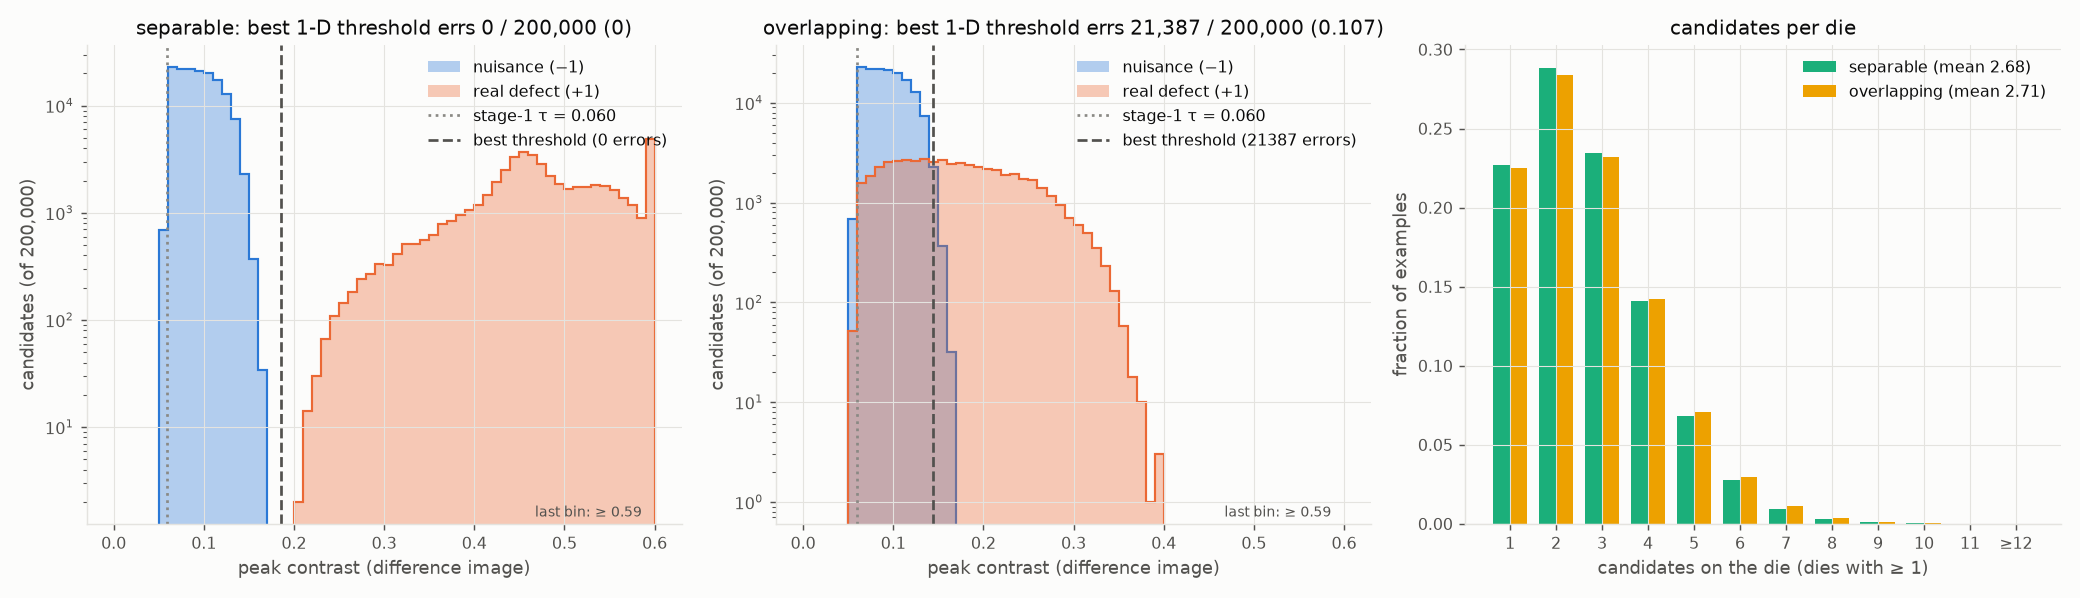
\includegraphics[width=0.8\linewidth]{../figures/stage1_regimes.png}
  \caption{Peak contrast of nuisance and real-defect candidates in the two regimes (population
  pool) and candidates per die.}
  \label{fig:regimes}
\end{figure}

\section{Result 1: a threshold on peak contrast}
\label{sec:result-1}

$\cH=\{h_\theta\}$ with $h_\theta(x)=+1$ iff $x>\theta$, on the scalar peak contrast $x$ (the
maximum of the difference image over the candidate). The learner is exact ERM: sort the $n$
training values, sweep the $n+1$ cuts with cumulative sums, and put $\hat\theta$ at the midpoint
of the chosen gap. $L(h)=\P_Q(h(x)\ne y)$ and $\hat L_S(h)$ is the training error.

$\cH$ has VC dimension $d=1$: one point is shattered ($\theta$ below or above it), but for
$x_1<x_2$ the labelling $(+1,-1)$ would need $x_1>\theta\ge x_2$. By the Sauer--Shelah lemma the
growth function, the number of labellings $\cH$ induces on $m\ge d$ points, satisfies
$\Pi_\cH(m)\le(em/d)^d$; for thresholds, $\Pi_\cH(2n)\le2en$.

\begin{theorem}[Result 1]
\label{thm:1}
Let $\hat h$ be any ERM hypothesis on $n$ i.i.d.\ examples from $Q$, and $h^\star\in\argmin_\cH L$.
\begin{enumerate}[label=(\roman*)]
  \item (Realizable.) If $L(h^\star)=0$ and $0<\delta\le1/2$, then with probability at least
  $1-\delta$
  \[ L(\hat h)\le\frac{2}{n\ln 2}\Bigl(\ln(2en)+\ln\frac2\delta\Bigr). \]
  \item (Agnostic.) With probability at least $1-\delta$
  \[ L(\hat h)-L(h^\star)\le\sqrt{\frac{32\bigl(\ln(2en)+\ln(4/\delta)\bigr)}{n}}. \]
\end{enumerate}
\end{theorem}

Both parts compare the training sample $S$ with an independent ghost sample $S'$ of size $n$.

\begin{lemma}[Uniform convergence]
\label{lem:uc}
For any class $\cH$ of binary classifiers and $n\epsilon^2\ge2$,
\[ \P\Bigl(\sup_{h\in\cH}\abs{L(h)-\hat L_S(h)}>\epsilon\Bigr)\le4\,\Pi_\cH(2n)\,e^{-n\epsilon^2/8}. \]
\end{lemma}
\begin{proof}
The argument goes back to \citet{vapnik1971uniform}; see also \citet{shalevshwartz2014understanding}.
\emph{Symmetrization.} On the event, pick (as a function of $S$) an $h$ with
$\abs{L(h)-\hat L_S(h)}>\epsilon$. Given $S$, $\hat L_{S'}(h)$ is a mean of $n$ independent
indicators with mean $L(h)$ and variance at most $1/(4n)$, so by Chebyshev
$\P(\abs{\hat L_{S'}(h)-L(h)}\ge\epsilon/2)\le1/(n\epsilon^2)\le1/2$. With probability at least
$1/2$ the two deviations therefore leave $\abs{\hat L_S(h)-\hat L_{S'}(h)}>\epsilon/2$, and
$\P(\sup_h\abs{L-\hat L_S}>\epsilon)\le2\,\P(\sup_h\abs{\hat L_S-\hat L_{S'}}>\epsilon/2)$.
\emph{Swaps.} All $2n$ points are i.i.d., so swapping the $i$-th points of $S$ and $S'$ does not
change the joint law of $(S,S')$, and after conditioning on the $2n$ points a hypothesis matters only
through its labelling of them. Let $\sigma_i=\pm1$ be independent fair signs that swap pair $i$ when $-1$. For a
fixed labelling with losses $a_i,b_i\in\{0,1\}$ on the $i$-th points of $S,S'$,
$\hat L_S-\hat L_{S'}=\frac1n\sum_i\sigma_i(a_i-b_i)$ is a sum of independent terms, each in an
interval of length at most $2/n$, so Hoeffding's inequality gives
$\P(\abs{\cdot}>\epsilon/2)\le2\exp\bigl(-2(\epsilon/2)^2/(n(2/n)^2)\bigr)=2e^{-n\epsilon^2/8}$.
A union bound over the at most $\Pi_\cH(2n)$ labellings and the factor 2 above give the claim.
\end{proof}

\begin{proof}[Proof of \cref{thm:1}]
(i) Let $\epsilon$ be the right-hand side of (i) and $A=\{\exists h:\hat L_S(h)=0,\ L(h)>\epsilon\}$.
Since $L(h^\star)=0$, $h^\star$ is consistent with $S$ almost surely, so every ERM hypothesis is
consistent and $L(\hat h)>\epsilon$ only on $A$.
\emph{Symmetrization.} On $A$, pick a consistent $h$ with $L(h)>\epsilon$. Given $S$, its number
of mistakes on $S'$ is binomial with mean $nL(h)>n\epsilon$ and variance below $nL(h)$, so by
Chebyshev it is below $nL(h)/2$ with probability at most $4/(nL(h))<4/(n\epsilon)\le1/2$, using
$n\epsilon=\frac{2}{\ln2}(\ln(2en)+\ln\frac2\delta)\ge\frac{2}{\ln2}(\ln(2e)+\ln4)>8$ for $n\ge1$,
$\delta\le\frac12$. Hence
$\P(A)\le2\,\P(\exists h:\hat L_S(h)=0,\ h\text{ errs on}\ge n\epsilon/2\text{ points of }S')$.
\emph{Swaps.} Fix the $2n$ points and a labelling with $k\ge n\epsilon/2$ mistakes. If some pair
$i$ holds two mistakes, $S$ always contains one. Otherwise the mistakes sit in $k$ different
pairs and all of them land in $S'$ with probability $2^{-k}\le2^{-n\epsilon/2}$.
\emph{Union bound.} $\P(A)\le2\,\Pi_\cH(2n)\,2^{-n\epsilon/2}\le2(2en)\exp\bigl(-\tfrac{n\epsilon\ln2}2\bigr)
=2(2en)\exp\bigl(-\ln(2en)-\ln\tfrac2\delta\bigr)=\delta$.

(ii) $L(\hat h)-L(h^\star)=[L(\hat h)-\hat L_S(\hat h)]+[\hat L_S(\hat h)-\hat L_S(h^\star)]+[\hat L_S(h^\star)-L(h^\star)]$,
and the middle term is $\le0$ for ERM, so the excess is at most $2\sup_h\abs{L(h)-\hat L_S(h)}$.
\Cref{lem:uc} at $\epsilon/2$ with $d=1$ gives $\P(L(\hat h)-L(h^\star)>\epsilon)\le4(2en)e^{-n\epsilon^2/32}$,
which equals $\delta$ at the right-hand side of (ii). The lemma's condition
$n(\epsilon/2)^2=8(\ln(2en)+\ln\frac4\delta)\ge2$ holds.
\end{proof}

\begin{inshort}
\begin{enumerate}[leftmargin=*]
  \item Thresholds have VC dimension 1, so $\Pi(2n)\le2en$.
  \item Realizable: a bad consistent $h$ makes $\ge n\epsilon/2$ mistakes on a ghost sample; random
    swaps put them all there with probability $\le2^{-n\epsilon/2}$; union over $2en$ labellings;
    solve for $\epsilon$: $\tilde O(1/n)$.
  \item Agnostic: excess $\le2\times$ uniform deviation; ghost sample, swaps and Hoeffding give
    $e^{-n\epsilon^2/32}$; union; solve: $\tilde O(1/\sqrt n)$.
  \item Both are worst cases over distributions: some distribution forces each rate, but a given
    one can be learned faster.
\end{enumerate}
\end{inshort}

\paragraph{Measured vs.\ theory (E1).} $\EOneRepeats$ repeats on fresh dies, $n=2^4,\dots,2^{14}$
(nested prefixes). $\hat h$ and $h^\star$ (ERM on the population pool) are evaluated on the same
test pool, so its noise largely cancels in the excess. Slopes are fitted where the mean is at
least $5\times$ the pool noise floor, and their ranges were fixed before running.

\begin{center}
\small
\begin{tabular}{lccc}
\toprule
regime & fitted slope (points) & range fixed in advance & bound above mean at every $n$ \\
\midrule
separable (test error) & $\EOneSepSlope$ ($\EOneSepFitPoints$) & $[-1.15,-0.85]$: \EOneSepSlopePass & \EOneSepBoundPass \\
overlapping (excess error) & $\EOneOvlSlope$ ($\EOneOvlFitPoints$) & $[-1.15,-0.45]$: \EOneOvlSlopePass & \EOneOvlBoundPass \\
\bottomrule
\end{tabular}
\end{center}

Both bounds hold in every run at every $n$, which is the test of the theory; the slopes are
descriptive. The overlapping excess falls faster than the worst case $n^{-1/2}$: the nuisance
density ends sharply at $\theta^\star$, where $P(\text{defect}\mid\text{contrast})$ jumps from
$\OvlCondBelow$ to $\OvlCondAbove$. Such a near-jump at the optimal threshold is consistent with the
faster measured rate; this is an observation, not something proved here.

\textbf{The separable slope check fails.} The separable pool has a gap: no candidate has peak
contrast in $(\SepMaxNuisancePeak,\SepMinDefectPeak)$. ERM puts $\hat\theta$ midway between the largest
nuisance and the smallest defect in its sample, and once that midpoint is in the gap the test
error is exactly zero: in $\EOneSepZeroFracSixteen$ of repeats at $n=16$, $\EOneSepZeroFracOneK$ at
$n=1024$, $\EOneSepZeroFracFourK$ at $n=4096$. The mean is carried by a shrinking set of unlucky runs
and falls faster than $1/n$ (fitted on only $\EOneSepFitPoints$ points). The bound is not
contradicted: $1/n$ is forced only by distributions with mass at the boundary, and a margin
makes learning faster. I kept the regime as designed and report the failure. The regime is also
only nearly realizable: $\theta^\star$ makes $\EOneSepTestErrors$ errors on $N=\EOneSepNTest$
independent test candidates, so $L(h^\star)\le\ln(1/\delta)/N=\EOneSepLStarBound$ with confidence
$1-\delta$ (as in \cref{sec:result-4}), and $\EOneSepInconsistentRuns$ of the $\EOneSepRunsTotal$
training samples is not separable. The proof of (i) only needs $\hat h$ to be consistent with its
sample, so (i) applies to every other run.

\begin{figure}[tb]
  \centering
  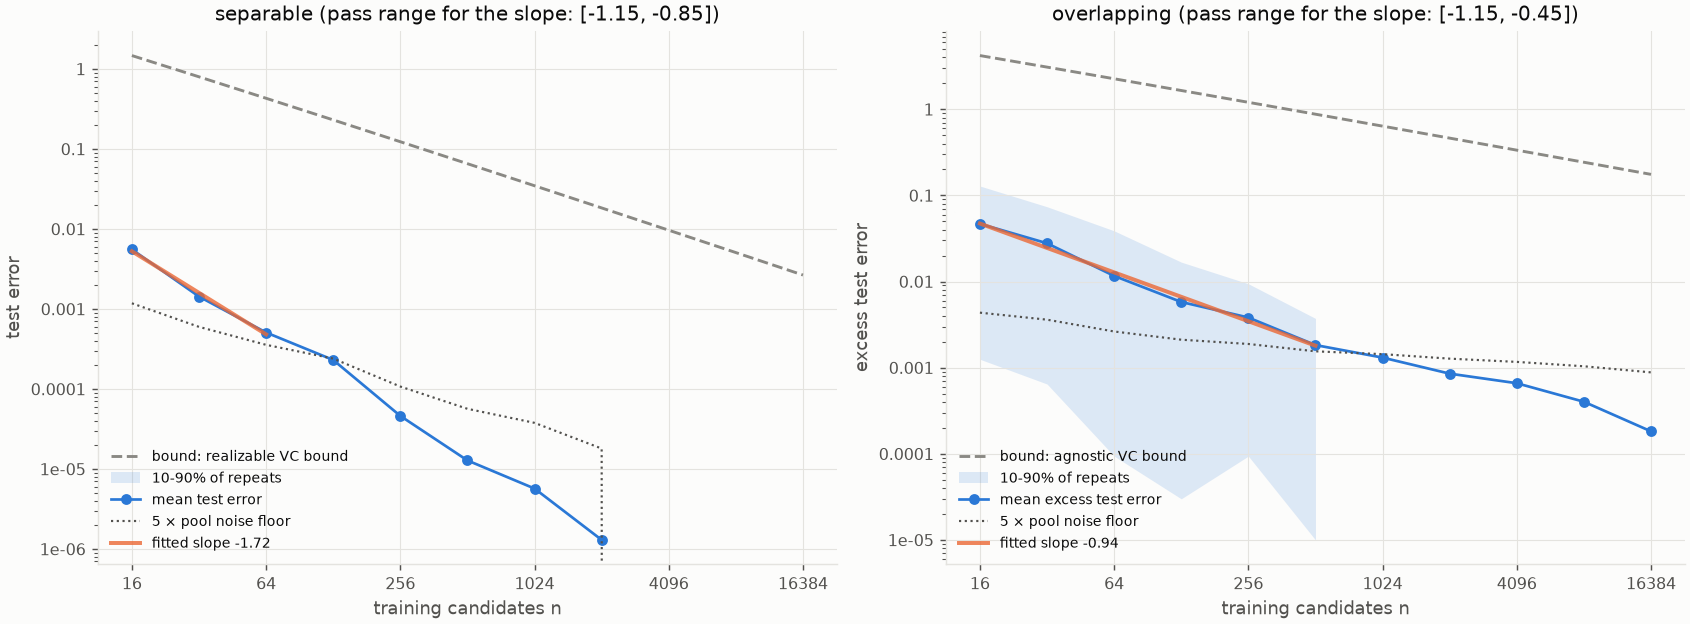
\includegraphics[width=0.8\linewidth]{../figures/e1_thresholds.png}
  \caption{E1: threshold ERM learning curves with the Result~1 bounds (dashed), the fitted slope
  and $5\times$ the pool noise floor. At $n=\EOneNLast$ the agnostic bound is
  $\EOneOvlBoundRatioLast\times$ the measured mean excess.}
  \label{fig:e1}
\end{figure}

\section{Result 2: VC and Rademacher bounds for the linear filter}
\label{sec:result-2}

Feature vectors $x\in\R^{k+1}$ ($k$ features and the intercept coordinate), $\norm{x}\le C=1$;
classifiers $x\mapsto\operatorname{sign}(w\cdot x)$; $L_{01}(w)=\P_Q(y\,w\cdot x\le0)$. The
logistic loss of the margin $u=y\,w\cdot x$ is $\ell(u)=\ln(1+e^{-u})$, and
$\psi(u)=\min(\ell(u),\ln2)$ is its clipped version; $\hat L$ denotes training averages. Training
always minimizes the logistic loss; $\psi$ is used only to evaluate the bound.

\begin{theorem}[Result 2]
\label{thm:2}
Let $S$ be $n$ i.i.d.\ examples from $Q$.
\begin{enumerate}[label=(\roman*)]
  \item (VC.) If $n\ge k+1$, with probability at least $1-\delta$, for every $w\in\R^{k+1}$,
  \[ L_{01}(w)\le\hat L_{01}(w)+\sqrt{\frac{8\bigl((k+1)\ln\frac{2en}{k+1}+\ln\frac4\delta\bigr)}{n}}. \]
  \item (Rademacher, clipped loss.) With probability at least $1-\delta$, for every $w$ with
  $\norm{w}\le B$,
  \[ L_{01}(w)\le\frac1{\ln2}\Bigl(\hat L_{\psi}(w)+\frac{2B}{n}\sqrt{\textstyle\sum_{i}\norm{x_i}^2}
     +3\ln2\,\sqrt{\frac{\ln(2/\delta)}{2n}}\Bigr). \]
  Applying (ii) at $\delta/G$ to each of $G$ grid values of $B$ makes all $G$ hold at once (union
  bound), so $B$ may be chosen after seeing the data.
\end{enumerate}
\end{theorem}

\begin{proof}
(i) Linear classifiers with an intercept on $\R^k$ have VC dimension $k+1$: the origin and the
$k$ unit vectors are shattered, and by Radon's theorem any $k+2$ points split into two sets whose
convex hulls intersect, so they cannot be separated. Our classifiers on $x=(z,1)$ are exactly
this class on $z\in\R^k$ (the convention at $w\cdot x=0$ does not change this). \Cref{lem:uc} with Sauer--Shelah, $\Pi(2n)\le(2en/d)^d$ for $d=k+1\le n$,
gives $\P(\sup_w\abs{L_{01}(w)-\hat L_{01}(w)}>\epsilon)\le4(2en/d)^de^{-n\epsilon^2/8}$. Setting
this to $\delta$ gives (i); the lemma's condition $n\epsilon^2\ge8\ln(4/\delta)\ge2$ holds.

(ii) Let $\cF=\{(x,y)\mapsto\psi(y\,w\cdot x):\norm{w}\le B\}$ and let
$\hat R_S(\cF)=\E_\sigma\sup_{f\in\cF}\frac1n\sum_i\sigma_if(z_i)$ be its empirical Rademacher
complexity, with independent fair signs $\sigma_i$.
\begin{enumerate}[label=(\alph*),leftmargin=*]
  \item \emph{Generalization bound.} If every $f\in\cF$ takes values in an interval of length
  $\Delta$, then with probability at least $1-\delta$, for all $f\in\cF$,
  $\E f\le\hat\E_Sf+2\hat R_S(\cF)+3\Delta\sqrt{\ln(2/\delta)/(2n)}$. Proof: changing one point
  changes $\Phi(S)=\sup_f(\E f-\hat\E_Sf)$ by at most $\Delta/n$, so McDiarmid's inequality \citep{mcdiarmid1989method} gives
  $\Phi(S)\le\E\Phi+\Delta\sqrt{\ln(2/\delta)/(2n)}$ with probability $1-\delta/2$. Symmetrization
  with a ghost sample and random signs (as in \cref{lem:uc}) gives $\E\Phi\le2\E\hat R_S(\cF)$.
  $\hat R_S(\cF)$ also changes by at most $\Delta/n$ per point, so McDiarmid again gives
  $\E\hat R_S\le\hat R_S+\Delta\sqrt{\ln(2/\delta)/(2n)}$ with probability $1-\delta/2$. A union
  bound over the two events gives the claim, which holds for all $f$ at once because it bounds
  the supremum.
  \item \emph{Range.} $\psi$ takes values in $(0,\ln2]$, so $\Delta\le\ln2$ for every $B$.
  \item \emph{Contraction.} $\abs{\ell'(u)}=1/(1+e^{u})\le1$, so $\ell$ is 1-Lipschitz, and so is
  $\psi$ ($\abs{\min(a,c)-\min(b,c)}\le\abs{a-b}$). By the contraction lemma of
  \citet[ch.~26]{shalevshwartz2014understanding} (if $\varphi_1,\dots,\varphi_n$ are $\rho$-Lipschitz,
  applying $\varphi_i$ to the $i$-th coordinate of every vector in a set $A\subset\R^n$ multiplies its
  Rademacher complexity by at most $\rho$; this version has no absolute values and needs no
  condition $\varphi_i(0)=0$), applied to the margin vectors $(y_i\,w\cdot x_i)_{i\le n}$ with
  $\varphi_i=\psi$, $\hat R_S(\cF)\le\hat R_S(\{(x,y)\mapsto y\,w\cdot x\})$.
  \item \emph{Margin class.} For fixed labels, $\sigma_iy_i$ are again independent fair signs, so
  the margin class has the same complexity as $\{x\mapsto w\cdot x:\norm w\le B\}$.
  \item \emph{Linear class.} By Cauchy--Schwarz, then Jensen, then $\E[\sigma_i\sigma_j]=\mathbb 1[i=j]$,
  \[ \E_\sigma\sup_{\norm w\le B}\frac1n\sum_i\sigma_i\,w\cdot x_i=\frac Bn\E_\sigma\Bigl\lVert\sum_i\sigma_ix_i\Bigr\rVert
     \le\frac Bn\Bigl(\E_\sigma\Bigl\lVert\sum_i\sigma_ix_i\Bigr\rVert^2\Bigr)^{1/2}=\frac Bn\sqrt{\textstyle\sum_i\norm{x_i}^2}. \]
  \item \emph{From $\psi$ to 0-1.} If $u\le0$ then $\ell(u)\ge\ell(0)=\ln2$, so $\psi(u)=\ln2$ and
  $\mathbb 1[u\le0]\le\psi(u)/\ln2$; hence $L_{01}(w)\le\E\psi/\ln2$.
\end{enumerate}
Combining (a)--(f) gives (ii). For the grid, each bound fails with probability at most $\delta/G$,
so all hold together with probability at least $1-\delta$, in particular for the chosen $B$.
\end{proof}

\begin{remark}[Unclipped version]
With $\ell$ in place of $\psi$ only step (b) changes: since $\abs{y\,w\cdot x}\le BC$ and
$\ln(1+e^{a})-\ln(1+e^{-a})=a$, $\ell$ ranges over an interval of length exactly $BC$, and the last
term becomes $3BC\sqrt{\ln(2/\delta)/(2n)}$, which grows with $B$. It is computed for comparison.
\end{remark}

\begin{inshort}
\begin{enumerate}[leftmargin=*]
  \item VC: half-spaces with intercept in $\R^k$ have $d=k+1$; plug into the uniform-convergence
    bound $4(2en/d)^de^{-n\epsilon^2/8}=\delta$. The gap is $\approx\sqrt{d\ln n/n}$: needs $n\gg d$.
  \item Rademacher: McDiarmid + symmetrization; clipped logistic loss has range $\le\ln2$ whatever
    $B$; contraction (1-Lipschitz); random signs absorb the labels; Cauchy--Schwarz + Jensen give
    $\frac Bn\sqrt{\sum\norm{x_i}^2}$; a mistake costs $\psi=\ln2$, so divide by $\ln2$.
    No dimension anywhere, only $B$ and the feature norms.
  \item A grid of $G$ values of $B$ costs $\ln G$ inside the square root.
\end{enumerate}
\end{inshort}

\paragraph{Measured vs.\ theory (E2a).} Overlapping regime; $\ETwoRepeats$ repeats on fresh dies,
$n=\ETwoNFirst,\dots,\ETwoNLast$. The projected-gradient fit runs at every $B\in\{2^{-1},\dots,2^8\}$
($G=10$) and $B$ is chosen by validation error; both bounds are evaluated for that filter. The
check fixed before running (both bounds above the test error in at least 95\% of runs) holds for
every feature set.

\begin{center}
\small
\resizebox{\linewidth}{!}{%
\begin{tabular}{lcccccccc}
\toprule
& & & \multicolumn{2}{c}{bound $\ge$ test error} & \multicolumn{2}{c}{first $n$ with bound $<\TrivialError$}
& \multicolumn{2}{c}{at $n=\ETwoNLast$} \\
\cmidrule(lr){4-5}\cmidrule(lr){6-7}\cmidrule(lr){8-9}
features & $k$ & $L(h^\star)$ & VC & Rad. & VC & Rad. & test error & VC / Rad.\ bound \\
\midrule
hand-crafted & 10 & $\ETwoHandLStar$ & \ETwoHandFracVC & \ETwoHandFracRad & $\ETwoHandFirstNVC$ & $\ETwoHandFirstNRad$ & $\ETwoHandTestLast$ & $\ETwoHandVCLast$ / $\ETwoHandRadLast$ \\
PCA-16 & 16 & $\ETwoPcaSixteenLStar$ & \ETwoPcaSixteenFracVC & \ETwoPcaSixteenFracRad & $\ETwoPcaSixteenFirstNVC$ & $\ETwoPcaSixteenFirstNRad$ & $\ETwoPcaSixteenTestLast$ & $\ETwoPcaSixteenVCLast$ / $\ETwoPcaSixteenRadLast$ \\
PCA-64 & 64 & $\ETwoPcaSixtyFourLStar$ & \ETwoPcaSixtyFourFracVC & \ETwoPcaSixtyFourFracRad & $\ETwoPcaSixtyFourFirstNVC$ & $\ETwoPcaSixtyFourFirstNRad$ & $\ETwoPcaSixtyFourTestLast$ & $\ETwoPcaSixtyFourVCLast$ / $\ETwoPcaSixtyFourRadLast$ \\
CNN-384 & 384 & $\ETwoCnnFullLStar$ & \ETwoCnnFullFracVC & \ETwoCnnFullFracRad & $\ETwoCnnFullFirstNVC$ & $\ETwoCnnFullFirstNRad$ & $\ETwoCnnFullTestLast$ & $\ETwoCnnFullVCLast$ / $\ETwoCnnFullRadLast$ \\
\bottomrule
\end{tabular}}
\end{center}

The VC bound beats the trivial error $\TrivialError$ only for the hand-crafted features (from
$n=\ETwoHandFirstNVC$); for CNN-384 it would need $n\approx\ETwoCnnFullVCNeedN$. The usual expectation
that the dimension-free bound is tighter fails: at the validated $B$ the Rademacher bound is
$\ETwoRadLastMin$--$\ETwoRadLastMax$, above VC for every feature set. Choosing $B$ to minimize the
Rademacher bound instead trades error for bound. For CNN-384 that filter's bound is tighter than VC
($\ETwoCnnFullRadCertLast$ vs $\ETwoCnnFullVCLast$), though neither is below the trivial $\TrivialError$,
and its test error is $\ETwoCnnFullRadCertTestLast$ instead of $\ETwoCnnFullTestLast$
(\cref{sec:looseness}).

\paragraph{Approximation vs.\ estimation (E2b).} $L(h^\star)$ is the test error of the logistic fit on
the population pool, an upper estimate of the best-in-class error. Richer CNN features lower it
and raise the estimation error at small $n$ (at $n=\ETwoNFirst$: $\ETwoPcaSixteenEstFirst$,
$\ETwoPcaSixtyFourEstFirst$, $\ETwoCnnFullEstFirst$ for PCA-16, PCA-64, CNN-384), so their curves
cross. The ten hand-crafted features match CNN-384's $L(h^\star)$ ($\ETwoHandLStar$ vs.\
$\ETwoCnnFullLStar$) with an estimation error of only $\ETwoHandEstFirst$ at $n=\ETwoNFirst$, and are
best at every $n$ tested.

\begin{figure}[tb]
  \centering
  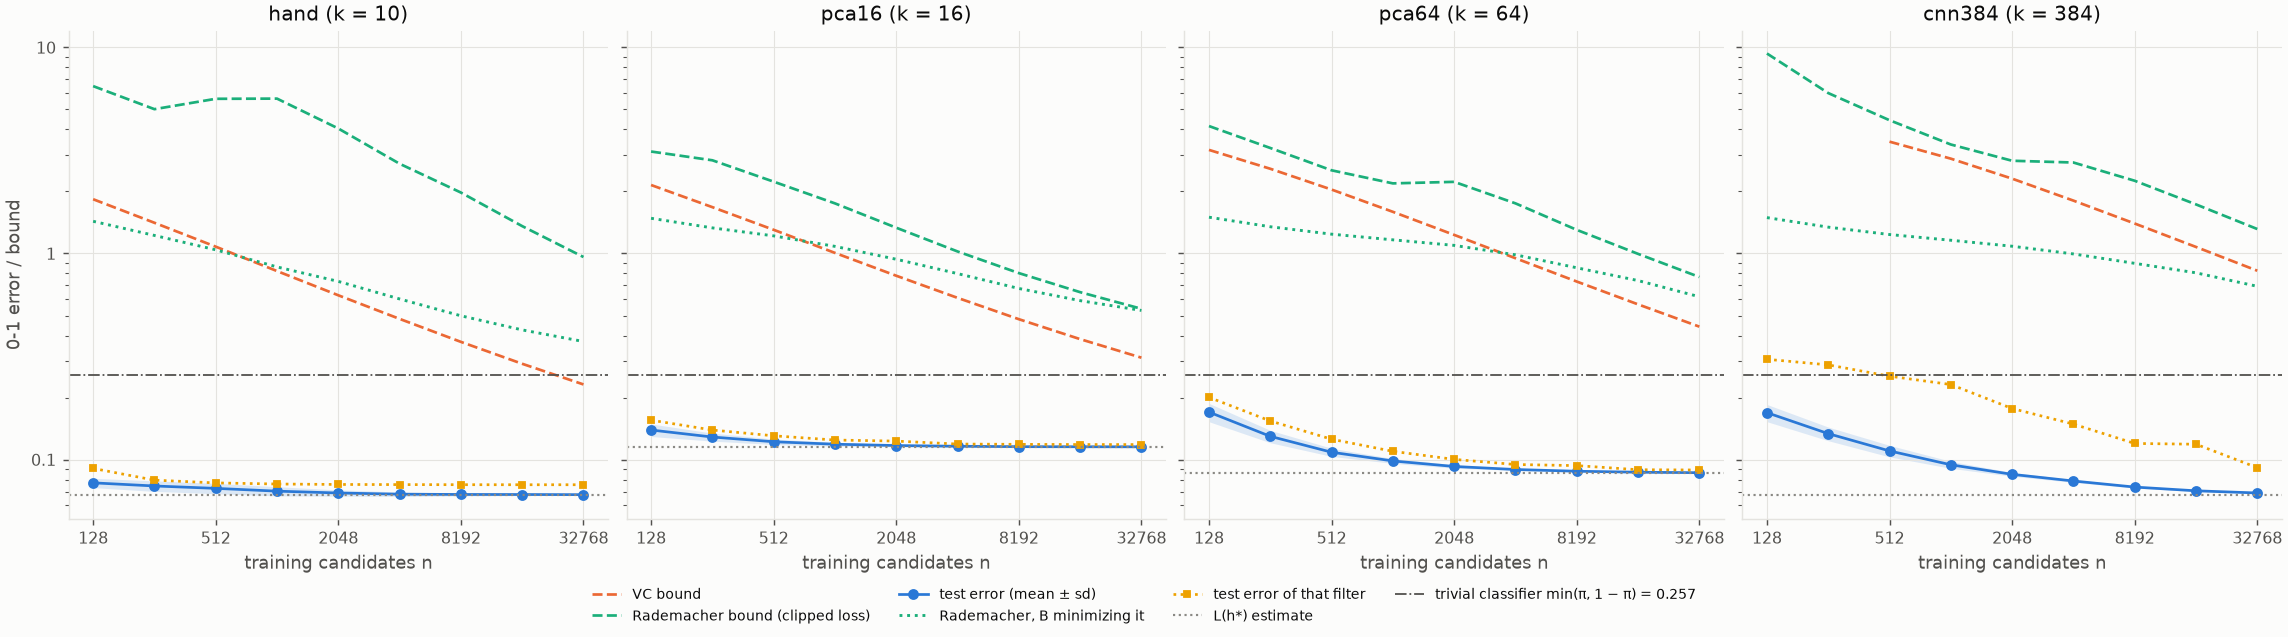
\includegraphics[width=0.8\linewidth]{../figures/e2a_bounds.png}\\[4pt]
  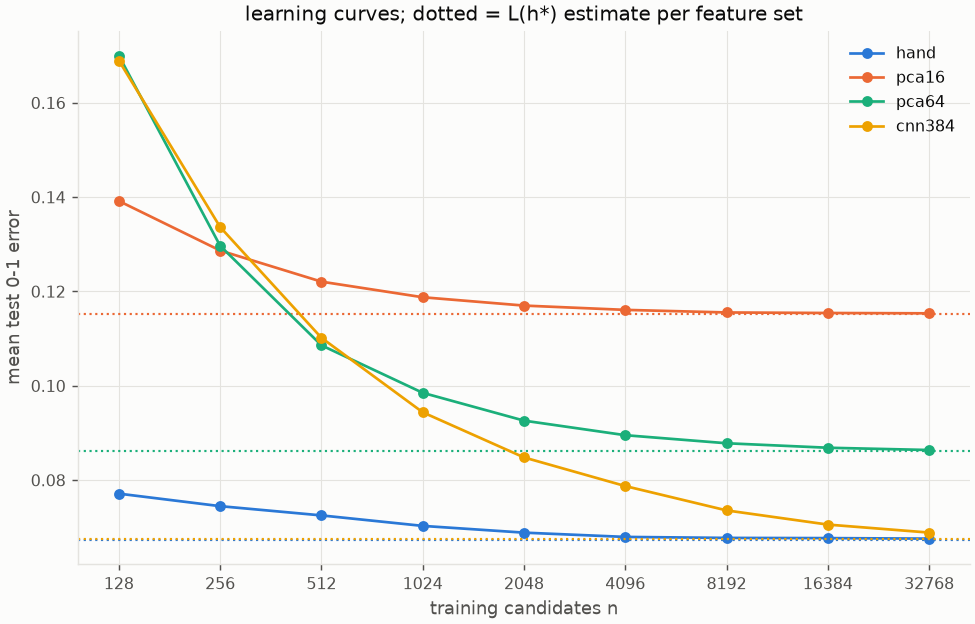
\includegraphics[width=0.5\linewidth]{../figures/e2b_curves.png}
  \caption{Top (E2a): test error and both Result~2 bounds per feature set; dash-dotted: the
  trivial error $\min(\pi,1-\pi)$. Bottom (E2b): learning curves with the $L(h^\star)$ estimates
  (dotted).}
  \label{fig:e2}
\end{figure}

\section{Result 3: the learning curve of logistic regression}
\label{sec:result-3}

Unregularized logistic regression: $\hat\theta_n=\argmin_\theta\hat L_n(\theta)$,
$\hat L_n(\theta)=\frac1n\sum_i\ell(\theta;x_i,y_i)$, $\ell(\theta;x,y)=\ln(1+e^{-y\,\theta\cdot x})$,
$\theta\in\R^p$ ($p=k+1$), $\phi$ the sigmoid, $L(\theta)=\E_Q\ell(\theta;x,y)$ and
$\theta^\star=\argmin L$. Unlike Results~1 and 2 this is not a bound but a prediction of the
learning curve itself.

\begin{theorem}[Result 3]
\label{thm:3}
Let $H=\E[\phi(\theta^\star\cdot x)\phi(-\theta^\star\cdot x)\,xx^\top]$ and $G=\E[\nabla\ell\,\nabla\ell^\top]$
at $\theta^\star$, with $\nabla\ell=-\phi(-y\,\theta^\star\cdot x)\,y\,x$. If $\theta^\star$ exists,
$\hat\theta_n\to\theta^\star$ in probability and $H\succ0$, then
\[ \sqrt n(\hat\theta_n-\theta^\star)\xrightarrow{d}N(0,H^{-1}GH^{-1}),\qquad
   n\bigl(L(\hat\theta_n)-L(\theta^\star)\bigr)\xrightarrow{d}\tfrac12Z^\top HZ,\quad Z\sim N(0,H^{-1}GH^{-1}), \]
and the limit has mean $\Tr(H^{-1}G)/2$, which gives the prediction
$\E[L(\hat\theta_n)-L(\theta^\star)]\approx\Tr(H^{-1}G)/(2n)$. If the model is well specified,
$G=H$ and the prediction is $p/(2n)$, so $\Tr(H^{-1}G)/p$ measures misspecification.
\end{theorem}

\begin{proof}
\emph{Derivatives.} With $t=\theta\cdot x$, $\frac{d}{dt}\ln(1+e^{-yt})=-y\,\phi(-yt)$, so
$\nabla\ell=-\phi(-y\,\theta\cdot x)\,y\,x$; differentiating again and using $y^2=1$ and
$\phi(-yt)\phi(yt)=\phi(t)\phi(-t)$, $\nabla^2\ell=g(\theta\cdot x)\,xx^\top$ with $g(t)=\phi(t)\phi(-t)$.
Its expectation at $\theta^\star$ is $H$.

\emph{Assumptions.} $\theta^\star$ exists because the population is not linearly separable (the
classes overlap); training samples that \emph{are} separable have no minimizer and are excluded.
Consistency of $\hat\theta_n$ is the standard consistency of M-estimators \citep{vandervaart1998asymptotic}; here
$\hat L_n$ is convex and $\theta^\star$ is unique because $\nabla^2L\succ0$ everywhere.
$H\succ0$ because the features are not supported on a hyperplane and $g>0$. $G$ is finite because
$\norm{\nabla\ell}\le\norm x\le1$. The Hessian is Lipschitz: $g'=g(1-2\phi)$ and $\abs{g'}\le1/(6\sqrt3)\le1$,
so $\norm{\nabla^2\ell(\theta)-\nabla^2\ell(\theta')}\le\abs{(\theta-\theta')\cdot x}\norm x^2\le\norm{\theta-\theta'}$.

\emph{Asymptotic normality.} Since $\nabla\hat L_n(\hat\theta_n)=0$, Taylor's theorem in integral
form gives $0=\nabla\hat L_n(\theta^\star)+\bar H_n(\hat\theta_n-\theta^\star)$ with
$\bar H_n=\int_0^1\nabla^2\hat L_n(\theta^\star+s(\hat\theta_n-\theta^\star))\,ds$. By the Lipschitz
bound, $\norm{\bar H_n-\nabla^2\hat L_n(\theta^\star)}\le\norm{\hat\theta_n-\theta^\star}\to0$, and
$\nabla^2\hat L_n(\theta^\star)\to H$ by the law of large numbers, so $\bar H_n\to H$ in probability
and is invertible with probability tending to 1. The summands of $\nabla\hat L_n(\theta^\star)$
are i.i.d.\ with mean $\nabla L(\theta^\star)=0$ and covariance $G$, so by the central limit
theorem $\sqrt n\,\nabla\hat L_n(\theta^\star)\to N(0,G)$, and by Slutsky's lemma
$\sqrt n(\hat\theta_n-\theta^\star)=-\bar H_n^{-1}\sqrt n\,\nabla\hat L_n(\theta^\star)\to N(0,H^{-1}GH^{-1})$:
the sandwich covariance.

\emph{Excess risk.} $\nabla L(\theta^\star)=0$ and $\nabla^2L$ is Lipschitz with constant 1, so
with $v=\hat\theta_n-\theta^\star$,
\[ \abs{L(\hat\theta_n)-L(\theta^\star)-\tfrac12v^\top Hv}\le\tfrac16\norm v^3. \]
Multiplying by $n$, the remainder is $O_P(n^{-1/2})$ and $n\cdot\frac12v^\top Hv\to\frac12Z^\top HZ$ by
the continuous mapping theorem. Its mean is $\frac12\Tr(H\,H^{-1}GH^{-1})=\frac12\Tr(H^{-1}G)$.
Reading this limit mean as the mean of $n(L(\hat\theta_n)-L(\theta^\star))$ at finite $n$ is the
approximation that the experiment tests.

\emph{Well specified.} If $P(y=1\mid x)=\phi(\theta^\star\cdot x)$, then with $t=\theta^\star\cdot x$,
$\E[\phi(-yt)^2\mid x]=\phi(t)\phi(-t)^2+\phi(-t)\phi(t)^2=\phi(t)\phi(-t)$, so $G=H$ and
$\Tr(H^{-1}G)=p$.
\end{proof}

\begin{inshort}
\begin{enumerate}[leftmargin=*]
  \item Gradient $-\phi(-y\theta\cdot x)yx$, Hessian $\phi\phi\,xx^\top$, Lipschitz because $\norm x\le1$.
  \item One Newton step from $\theta^\star$: $\hat\theta-\theta^\star\approx-H^{-1}\nabla\hat L(\theta^\star)$;
    CLT on the gradient (mean 0, covariance $G/n$) gives the sandwich $H^{-1}GH^{-1}/n$.
  \item The excess risk is half the squared $H$-norm: $\frac12\E\,v^\top Hv=\Tr(H^{-1}G)/2n$.
  \item Well specified $\Rightarrow G=H\Rightarrow p/2n$.
\end{enumerate}
\end{inshort}

\paragraph{Measured vs.\ theory (E3).} Overlapping regime; PCA-$k$ CNN features, $k\in\{4,16,64\}$;
$\EThreeRepeats$ repeats on fresh dies, $n\in\{10,20,50,100,300\}\times p$. $\theta^\star$ is fitted on
$\EThreeNPop$ population candidates (which biases the measured excess low by at most
$\EThreePopBias$), $H$ and $G$ on the disjoint test pool. The measured quantity is
$n(L_{\text{test}}(\hat\theta_n)-L_{\text{test}}(\theta^\star))$. The check fixed before running,
measured/predicted in $[0.9,1.1]$ at the largest $n$, holds for all three feature sets.

\begin{center}
\small
\begin{tabular}{lccccccc}
\toprule
& & \multicolumn{2}{c}{prediction for $n\cdot$excess} & \multicolumn{2}{c}{measured at $n=300p$} & & \\
\cmidrule(lr){3-4}\cmidrule(lr){5-6}
features & $p$ & $\Tr(H^{-1}G)/2$ & $p/2$ & mean $\pm$ se & ratio & in $\pm10\%$ from & Wald cov. \\
\midrule
PCA-4 & $\EThreePcaFourP$ & $\EThreePcaFourPred$ & $\EThreePcaFourPHalf$ & $\EThreePcaFourMeasLast\pm\EThreePcaFourSeLast$ & $\EThreePcaFourRatioLast$ & $\EThreePcaFourFromNP\,p$ & $\EThreePcaFourCoverage$ \\
PCA-16 & $\EThreePcaSixteenP$ & $\EThreePcaSixteenPred$ & $\EThreePcaSixteenPHalf$ & $\EThreePcaSixteenMeasLast\pm\EThreePcaSixteenSeLast$ & $\EThreePcaSixteenRatioLast$ & $\EThreePcaSixteenFromNP\,p$ & $\EThreePcaSixteenCoverage$ \\
PCA-64 & $\EThreePcaSixtyFourP$ & $\EThreePcaSixtyFourPred$ & $\EThreePcaSixtyFourPHalf$ & $\EThreePcaSixtyFourMeasLast\pm\EThreePcaSixtyFourSeLast$ & $\EThreePcaSixtyFourRatioLast$ & $\EThreePcaSixtyFourFromNP\,p$ & $\EThreePcaSixtyFourCoverage$ \\
\bottomrule
\end{tabular}
\end{center}

At $n=10p$ the measured excess is $\EThreePcaSixteenRatioFirst$--$\EThreePcaFourRatioFirst$ times the
prediction, and the ratio enters the $\pm10\%$ band from $n=\EThreePcaFourFromNP\,p$ to
$\EThreePcaSixteenFromNP\,p$. At $n=300p$ the sandwich covariance holds as well ($n$ times the
covariance of $\hat\theta_n$ over the repeats has $\EThreePcaFourCovTraceLast$--$\EThreePcaSixtyFourCovTraceLast$
times the trace of $H^{-1}GH^{-1}$), and Wald intervals from each run's own sandwich estimate reach
nominal coverage (at $n=10p$ they under-cover, down to $\EThreePcaSixtyFourCoverageFirst$). The
model is mildly misspecified ($\Tr(H^{-1}G)/p=\EThreePcaFourMiss$--$\EThreePcaSixteenMiss$), so the
shortcut $p/2n$ would be off by under 10\%.

\begin{figure}[tb]
  \centering
  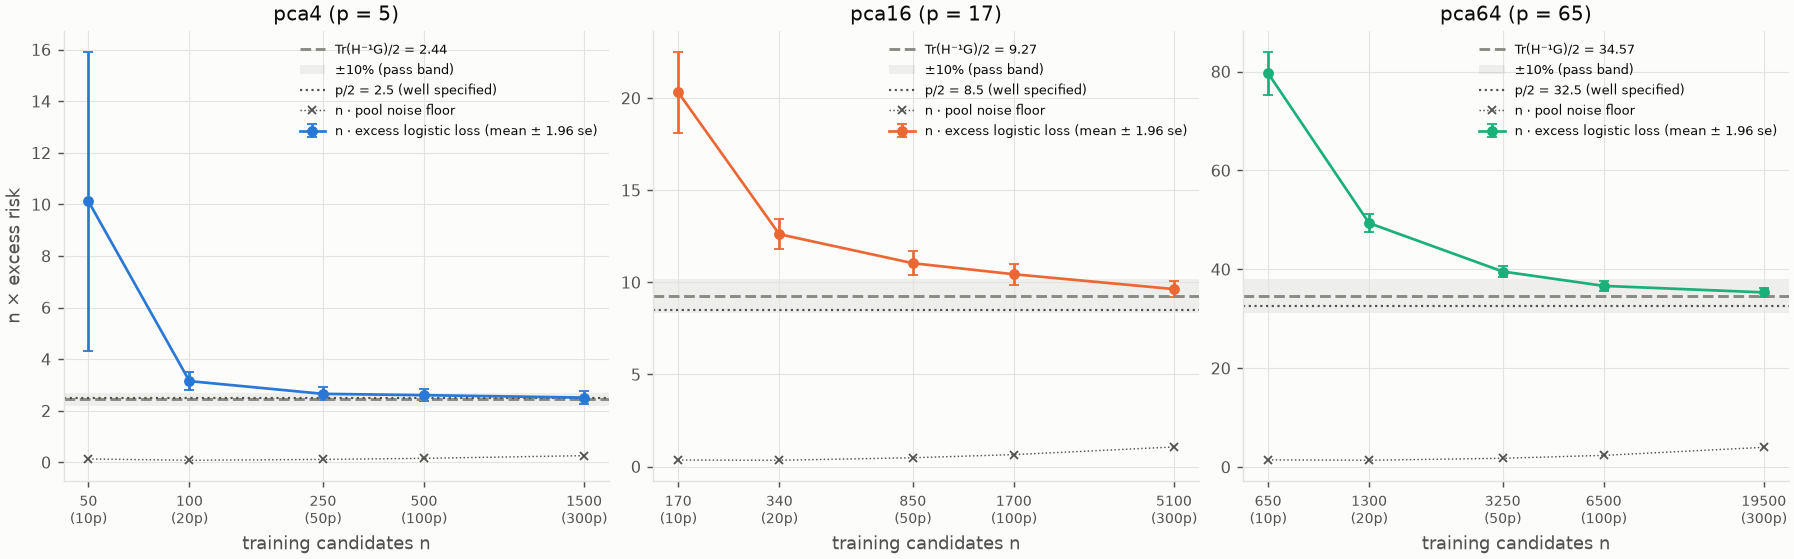
\includegraphics[width=0.8\linewidth]{../figures/e3_learning_curve.png}
  \caption{E3: $n\cdot$excess logistic loss (mean $\pm1.96$ se) with the prediction
  $\Tr(H^{-1}G)/2$ (dashed), its $\pm10\%$ band, $p/2$ (dotted) and $n$ times the pool noise floor.}
  \label{fig:e3}
\end{figure}

\subsection{Result 3b: what more labels will buy}
\label{sec:result-3b}

Result~3 needs $H$ and $G$ at $\theta^\star$, which are population quantities. With $n$ labels in
hand, the practical question is how much $m$ times as many would help. The difference of two
applications of \cref{thm:3} answers it, and the curvature it needs can be estimated from the
$n$ labels already collected.

\begin{proposition}[Result 3b]
\label{thm:3b}
Under the assumptions of \cref{thm:3}, let $m>1$ and let the $n$-sample be the first $n$ points
of the $mn$-sample. Then
$\E[L(\hat\theta_n)-L(\hat\theta_{mn})]\approx\frac{\Tr(H^{-1}G)}2\bigl(\frac1n-\frac1{mn}\bigr)$. With
\[ \hat H_n=\frac1n\sum_{i\le n}g(\hat\theta_n\cdot x_i)\,x_ix_i^\top,\qquad
   \hat G_n=\frac1n\sum_{i\le n}\nabla\ell(\hat\theta_n;x_i,y_i)\nabla\ell(\hat\theta_n;x_i,y_i)^\top, \]
$\Tr(\hat H_n^{-1}\hat G_n)\to\Tr(H^{-1}G)$ in probability, so the plug-in prediction
$\hat P_n=\frac12\Tr(\hat H_n^{-1}\hat G_n)(\frac1n-\frac1{mn})$ satisfies $n\hat P_n\to\frac{m-1}{2m}\Tr(H^{-1}G)$.
It predicts the expected improvement, not that of a single run.
\end{proposition}

\begin{proof}
\emph{Difference of two excess risks.} $L(\hat\theta_n)-L(\hat\theta_{mn})=[L(\hat\theta_n)-L(\theta^\star)]-
[L(\hat\theta_{mn})-L(\theta^\star)]$; take expectations and apply \cref{thm:3} at $n$ and at $mn$.
This is linearity of expectation, so the nesting does not affect the mean; it only makes the two
terms positively correlated, which lowers the variance of the measured difference.

\emph{Consistency of the plug-in.} Write $\hat H_n(\theta)$ for the average at $\theta$. Since
$\abs{g'}\le1$ and $\norm{x_ix_i^\top}=\norm{x_i}^2\le1$,
$\norm{\hat H_n(\theta)-\hat H_n(\theta')}\le\norm{\theta-\theta'}$, hence
$\norm{\hat H_n(\hat\theta_n)-H}\le\norm{\hat\theta_n-\theta^\star}+\norm{\hat H_n(\theta^\star)-H}$. The
first term tends to 0 by consistency, the second by the law of large numbers (bounded i.i.d.\
summands with mean $H$). For $\hat G_n$, $\nabla\ell\,\nabla\ell^\top=\phi(-y\,\theta\cdot x)^2xx^\top$ and
$\abs{\frac{d}{dt}\phi(-t)^2}=2\phi(-t)^2\phi(t)\le\frac8{27}\le1$ (the maximum of $2a^2(1-a)$, at
$a=\frac23$), so the same two steps give $\hat G_n\to G$. Since $H\succ0$, $(A,B)\mapsto\Tr(A^{-1}B)$
is continuous at $(H,G)$, and the continuous mapping theorem gives the claim.

\emph{Expected, not single-run.} By \cref{thm:3}, $n$ times one run's excess at $n$ converges to the
non-degenerate $\frac12Z^\top HZ$, and likewise at $mn$. Part of the improvement's spread comes from
the $(m-1)n$ labels not yet drawn, which are independent of the first $n$, so no function of the
first $n$ labels can predict it.
\end{proof}

\begin{inshort}
\begin{enumerate}[leftmargin=*]
  \item Excess at $n$ minus excess at $mn$: $\frac{\Tr(H^{-1}G)}2(\frac1n-\frac1{mn})$, i.e.\
    $\frac38\Tr(H^{-1}G)/n$ for $m=4$.
  \item Plug in $\hat H_n,\hat G_n$ at $\hat\theta_n$: Lipschitz in $\theta$ plus a law of large
    numbers at $\theta^\star$ makes them consistent.
  \item It predicts the mean; one run keeps an $O(1/n)$ spread that the first $n$ labels cannot remove.
\end{enumerate}
\end{inshort}

\paragraph{Measured vs.\ theory (E3b).} Same setup, $\EThreeBRepeats$ repeats,
$n\in\{\EThreeBNList\}\times p$, $m=\EThreeBFactor$. $\hat H_n,\hat G_n$ use the $n$ labels only; the
measured improvement is $L_{\text{test}}(\hat\theta_n)-L_{\text{test}}(\hat\theta_{\EThreeBFactor n})$. The
check fixed before running, mean prediction over mean measurement in
$[\EThreeBRangeLo,\EThreeBRangeHi]$ at the largest $n$, holds for all three feature sets.

\begin{center}
\small
\resizebox{\linewidth}{!}{%
\begin{tabular}{lcccccc}
\toprule
& \multicolumn{3}{c}{$n\cdot$improvement at $n=\EThreeBNMaxOverP\,p$} & & per-run error & 0-1 improvement \\
\cmidrule(lr){2-4}
features & measured & plug-in & population $H,G$ & plug-in / measured & sd / mean & (no theory) \\
\midrule
PCA-4 & $\EThreeBPcaFourMeasLast\pm\EThreeBPcaFourSeLast$ & $\EThreeBPcaFourPluginLast$ & $\EThreeBPcaFourPopLast$ & $\EThreeBPcaFourRatioLast$ & $\EThreeBPcaFourErrSd$ & $\EThreeBPcaFourZeroOneLast\pm\EThreeBPcaFourZeroOneSeLast$ \\
PCA-16 & $\EThreeBPcaSixteenMeasLast\pm\EThreeBPcaSixteenSeLast$ & $\EThreeBPcaSixteenPluginLast$ & $\EThreeBPcaSixteenPopLast$ & $\EThreeBPcaSixteenRatioLast$ & $\EThreeBPcaSixteenErrSd$ & $\EThreeBPcaSixteenZeroOneLast\pm\EThreeBPcaSixteenZeroOneSeLast$ \\
PCA-64 & $\EThreeBPcaSixtyFourMeasLast\pm\EThreeBPcaSixtyFourSeLast$ & $\EThreeBPcaSixtyFourPluginLast$ & $\EThreeBPcaSixtyFourPopLast$ & $\EThreeBPcaSixtyFourRatioLast$ & $\EThreeBPcaSixtyFourErrSd$ & $\EThreeBPcaSixtyFourZeroOneLast\pm\EThreeBPcaSixtyFourZeroOneSeLast$ \\
\bottomrule
\end{tabular}}
\end{center}

Estimating $H$ and $G$ from the $n$ labels costs almost nothing: plug-in and population predictions
agree within $\EThreeBMaxRatioGap$ (in ratio) at every $n$. What fails at small $n$ is the
asymptotic formula itself: at $n=\EThreeBNMinOverP\,p$ the prediction is only
$\EThreeBRatioFirstMin$--$\EThreeBRatioFirstMax$ of the improvement, because the excess at $n$ is still
far above its limit. Single runs scatter: the per-run error is as wide as the spread of the
improvement itself, while the prediction varies by only $\EThreeBPredSdMin$--$\EThreeBPredSdMax$ of the
mean. For PCA-4, $\EThreeBPcaFourFracNeg$ of runs even got worse with $\EThreeBFactor\times$ the labels.
The last column is the measured drop in test 0-1 error from $n$ to $\EThreeBFactor n$ labels (mean
$\pm$ se), reported with no theory attached.

\begin{figure}[tb]
  \centering
  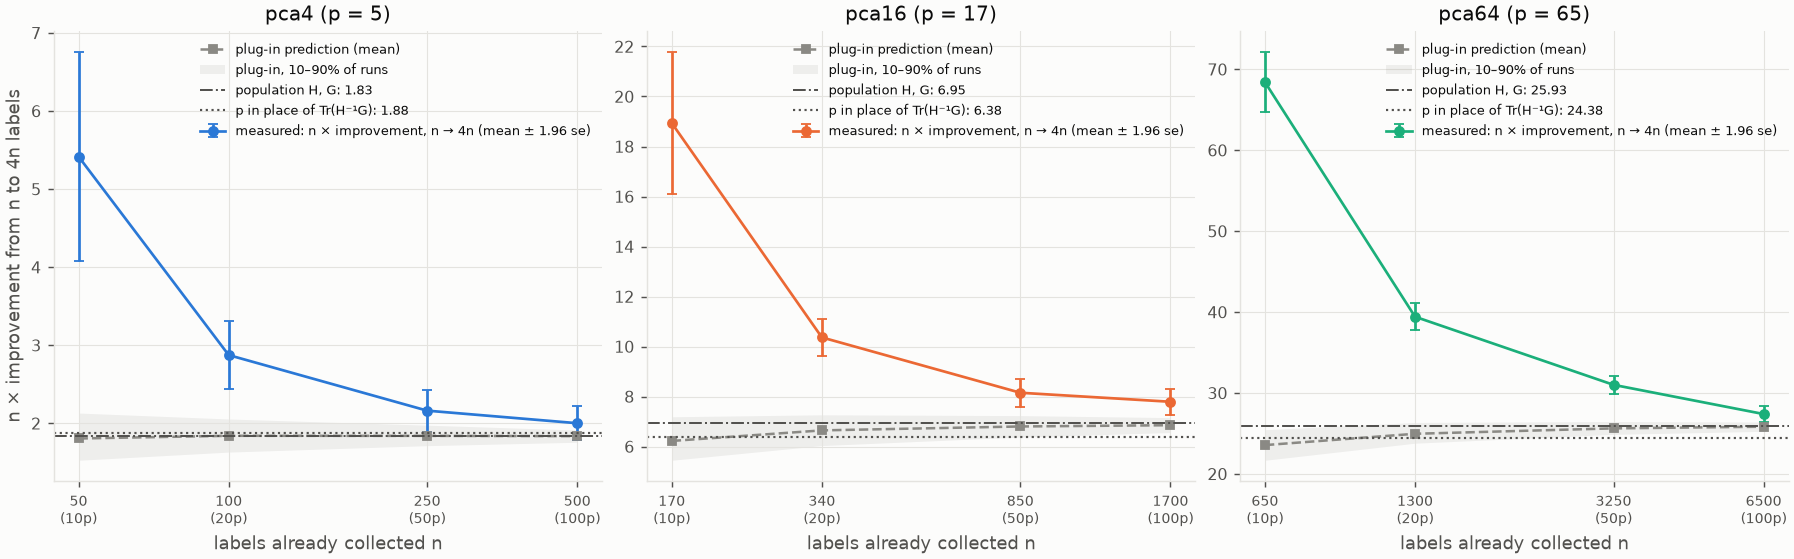
\includegraphics[width=0.8\linewidth]{../figures/e3b_plugin_curve.png}
  \caption{E3b: $n\cdot[L_{\text{test}}(\hat\theta_n)-L_{\text{test}}(\hat\theta_{\EThreeBFactor n})]$
  (mean $\pm1.96$ se), the plug-in prediction (mean and 10--90\% of runs), the same prediction
  with the population $H$, $G$ (dash-dotted) and with $p$ in place of $\Tr(H^{-1}G)$ (dotted).}
  \label{fig:e3b}
\end{figure}

\section{Result 4: certifying the die-level false-alarm rate}
\label{sec:result-4}

A frozen stage-2 scorer gives every candidate a score, and a die is flagged at threshold $t$ iff
some candidate's score exceeds $t$. $p(t)$ is the probability that a defect-free die is flagged,
and $\hat p_m(t)$ the fraction of $m$ i.i.d.\ defect-free certification dies that are flagged.

\begin{theorem}[Result 4]
\label{thm:4}
For a grid $t_1<\dots<t_T$ fixed before the certification dies are drawn, with probability at
least $1-\delta$, simultaneously for all $j$,
\[ p(t_j)\le\hat p_m(t_j)+\sqrt{\frac{\ln(T/\delta)}{2m}}. \]
So the selected threshold $\hat t$, the lowest $t_j$ whose right-hand side is at most $\alpha$,
satisfies $p(\hat t)\le\alpha$ with probability at least $1-\delta$ (if no $t_j$ qualifies, nothing
is certified).
\end{theorem}

\begin{proof}
Fix $j$. The flags $X_i=\mathbb 1[\text{die }i\text{ flagged at }t_j]$ are independent
Bernoulli$(p(t_j))$, because the dies are i.i.d.\ and the scorer and grid are fixed. Hoeffding's
inequality \citep{hoeffding1963probability} for the $[0,1]$-valued variables $1-X_i$ gives
$\P\bigl(\frac1m\sum_i(1-X_i)-(1-p(t_j))\ge\epsilon\bigr)\le e^{-2m\epsilon^2}$, that is,
$\P(p(t_j)-\hat p_m(t_j)\ge\epsilon)\le e^{-2m\epsilon^2}$. By the union bound over the $T$ grid points,
$\P(\exists j:p(t_j)-\hat p_m(t_j)\ge\epsilon)\le Te^{-2m\epsilon^2}$, which equals $\delta$ at
$\epsilon=\sqrt{\ln(T/\delta)/(2m)}$. On the complementary event every $t_j$ obeys the inequality,
in particular the data-dependent $\hat t$, whose right-hand side is $\le\alpha$ by construction.
\end{proof}

\begin{inshort}
\begin{enumerate}[leftmargin=*]
  \item Each threshold's false-alarm count is a sum of i.i.d.\ coin flips: one-sided Hoeffding,
    $e^{-2m\epsilon^2}$.
  \item The threshold is chosen from the data, so protect all $T$ at once: union bound,
    $Te^{-2m\epsilon^2}=\delta$. Choosing costs $\ln T$ under the square root.
  \item The grid must be fixed before the certification dies are seen (here: from the validation pool).
\end{enumerate}
\end{inshort}

\paragraph{Measured vs.\ theory (E4).} Overlapping regime; $\alpha=\EFourAlpha$, $\delta=0.05$,
$T=\EFourT$. Fixed before any certification die is drawn: the scorer (norm-constrained logistic
regression on the hand-crafted features, trained once on $\EFourNTrain$ candidates, $B=\EFourScorerB$
by validation, validation error $\EFourScorerValError$) and the grid (quantiles of the validation
pool's nuisance scores). Each of $R=\EFourRepeats$ repeats uses fresh defect-free dies. The true
false-alarm rate is the flag frequency on the far-test pool ($\EFourNFar$ dies). The check fixed
before running, a violation fraction $\le\delta$ at every $m$, holds.

\begin{center}
\small
\begin{tabular}{rccccc}
\toprule
$m$ & margin $\sqrt{\ln(T/\delta)/2m}$ & certifiable & certified bound & true FAR & defective dies flagged \\
\midrule
500 & $\EFourFiveHundredMargin$ & \EFourFiveHundredCert & $\EFourFiveHundredCertBound$ & $\EFourFiveHundredTrueFar$ & $\EFourFiveHundredDetect$ \\
1{,}000 & $\EFourOneKMargin$ & \EFourOneKCert & $\EFourOneKCertBound$ & $\EFourOneKTrueFar$ & $\EFourOneKDetect$ \\
2{,}000 & $\EFourTwoKMargin$ & \EFourTwoKCert & $\EFourTwoKCertBound$ & $\EFourTwoKTrueFar$ & $\EFourTwoKDetect$ \\
4{,}000 & $\EFourFourKMargin$ & \EFourFourKCert & $\EFourFourKCertBound$ & $\EFourFourKTrueFar$ & $\EFourFourKDetect$ \\
8{,}000 & $\EFourEightKMargin$ & \EFourEightKCert & $\EFourEightKCertBound$ & $\EFourEightKTrueFar$ & $\EFourEightKDetect$ \\
\bottomrule
\end{tabular}

{\small Certified bound, true FAR and detection are means over the repeats that certified.}
\end{center}

No repeat selected a threshold whose true rate exceeds $\alpha$ (largest: $\EFourMaxSelectedFar$).
Given the scorer, grid and far-test pool, the repeats' violation indicators are i.i.d.\
Bernoulli$(q)$, and zero violations have probability $(1-q)^R\le e^{-qR}<\delta$ whenever
$q>\ln(1/\delta)/R$; so with confidence $1-\delta$ the violation rate is at most
$\ln(1/\delta)/R=\EFourViolBoundZero$, below $\delta$ as the theorem says.

Nothing can be certified below $m=\EFourMinMPossible$, where the margin alone exceeds $\alpha$;
$m=\EFourSmallestM$ certifies in every repeat. Since the rule leaves room for the margin, the
selected thresholds land far below $\alpha$, and more dies buy sensitivity: detection
$\EFourTwoKDetect$ at $m=2{,}000$ and $\EFourEightKDetect$ at $m=8{,}000$, against $\EFourOracleDetect$
for the threshold one would pick knowing $p(t)$.

\begin{figure}[tb]
  \centering
  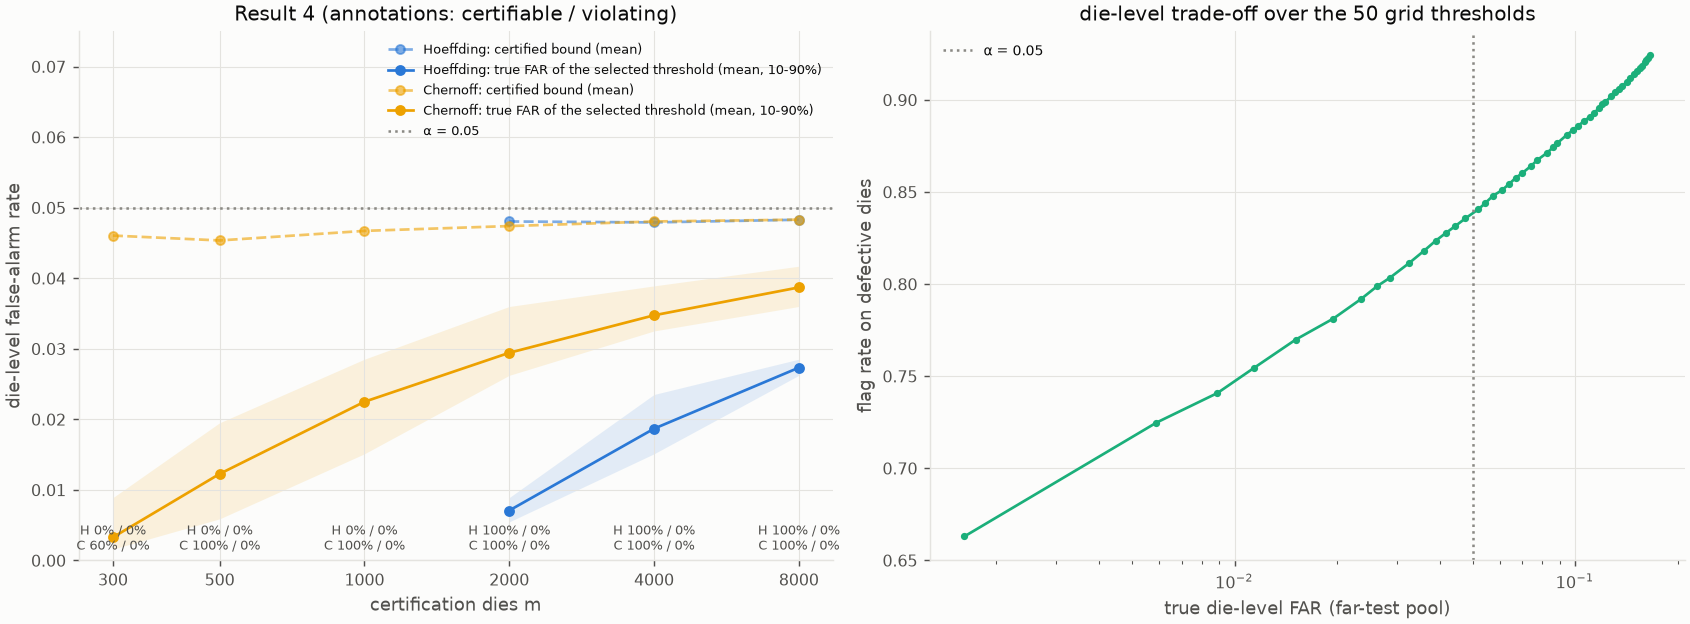
\includegraphics[width=0.8\linewidth]{../figures/e4_false_alarms.png}
  \caption{E4: certified bound and true false-alarm rate of the selected threshold vs.\ $m$
  (left; annotations: fraction of repeats that certified and that violated), and the die-level
  trade-off over the grid (right).}
  \label{fig:e4}
\end{figure}

\section{Where the bounds are loose}
\label{sec:looseness}

Every guarantee held in every experiment, and the asymptotic prediction matched. The bounds are
still loose by very different factors, and each gap traces back to one step of its proof.

\paragraph{Result 1, agnostic: the worst case.} At $n=\EOneNLast$ the bound is
$\EOneOvlBoundRatioLast\times$ the measured mean excess. (i) \emph{Rate:} it decays like
$\sqrt{\ln n/n}$ because it must hold for every distribution, while the measured excess decays like
$n^{\EOneOvlSlope}$. (ii) \emph{Constants:} the factor 2 for the excess and the ghost-sample halving give the 32 in
$e^{-n\epsilon^2/32}$. (iii) \emph{Counting:} the union bound runs over all $2en$ labellings of the
double sample, though only thresholds near $\theta^\star$ ever compete.

\paragraph{Result 2, VC: dimension against sample size.} The gap grows like $\sqrt{(k+1)\ln n/n}$, so
the bound says nothing until $n$ is many times $k+1$. For the ten hand-crafted features it is
$\ETwoHandVCRatioLast\times$ the measured error at $n=\ETwoNLast$, the tightest bound here; for CNN-384
it stays above the trivial error over the whole range.

\paragraph{Result 2, Rademacher: the norm of the weights.} At $n=\ETwoNLast$ and the validated
$B$ (mean $\ETwoHandBMeanLast$ for the hand-crafted features, $\norm{w^\star}=\ETwoHandWStar$), the
hand-crafted bound $\ETwoHandRadLast$ splits into training loss $\ETwoHandTrainPsiTermLast$, complexity
term $\ETwoHandCompTermLast$ and deviation term $\ETwoDevTermLast$ (CNN-384: $\ETwoCnnFullTrainPsiTermLast$,
$\ETwoCnnFullCompTermLast$, $\ETwoDevTermLast$; unclipped bounds $\ETwoHandRadUnclippedLast$ and
$\ETwoCnnFullRadUnclippedLast$). Clipping keeps the McDiarmid term at $\ETwoDevTermLast$ whatever $B$; with the logistic loss it pays
the range $BC$ and alone reaches $\ETwoPcaSixteenDevTermUnclippedLast$--$\ETwoCnnFullDevTermUnclippedLast$.
The binding term is now the complexity term, which is large because $B$ is: a filter with
near-optimal logistic loss needs $\norm w$ near $\norm{w^\star}$, which is large because the classes
overlap, and validation picks $B$ of that order. The surrogate costs too: even with infinite data
the bound for $w^\star$ cannot go below $L_\psi(w^\star)/\ln2=\ETwoHandPsiFloor$--$\ETwoPcaSixteenPsiFloor$,
against $L(h^\star)=\ETwoHandLStar$--$\ETwoPcaSixteenLStar$. Up to constants the VC term is
$\sqrt{(k+1)\ln n/n}$ and the Rademacher term $Br/\sqrt n$, so Rademacher wins only when $Br$ is small
next to $\sqrt{(k+1)\ln n}$. Here $Br$ is $\ETwoHandBr$ vs.\ $\ETwoHandVCRoot$ (hand-crafted),
$\ETwoPcaSixteenBr$ vs.\ $\ETwoPcaSixteenVCRoot$ (PCA-16), $\ETwoPcaSixtyFourBr$ vs.\ $\ETwoPcaSixtyFourVCRoot$ (PCA-64) and
$\ETwoCnnFullBr$ vs.\ $\ETwoCnnFullVCRoot$ (CNN-384). The dimension-free bound suits high-dimensional
features with large-margin data, not this overlapping problem.

\paragraph{Result 3: not a bound.} The prediction is a limit, so it cannot be ``loose''. It is within
10\% from $n=\EThreePcaFourFromNP\,p$ to $\EThreePcaSixteenFromNP\,p$ depending on the features, and
underestimates the excess at $n=10p$ by up to $\EThreePcaFourRatioFirst\times$. Result~3b shows that
estimating $H$ and $G$ is not the weak point; the onset of the asymptotic regime is.

\paragraph{Result 4: the variance of rare flags and a union bound.} (i) Hoeffding's inequality
holds for every Bernoulli parameter, so its margin is the one for variance $\frac14$, while flags at
a rate near $\alpha=\EFourAlpha$ have variance about $\alpha$. The multiplicative Chernoff bound uses
that small variance: its margin is relative, $\eta\alpha$ with $\eta\propto1/\sqrt{\alpha m}$ instead of
$1/\sqrt m$, so it certifies from $m=\EFourChSmallestMAll$ in every repeat instead of
$\EFourSmallestM$, and detects $\EFourChTwoKDetect$ instead of $\EFourTwoKDetect$ at $m=2{,}000$.
Exact binomial intervals would be tighter still. (ii) The union over $T=\EFourT$ thresholds
widens Hoeffding's margin by $\sqrt{\ln(T/\delta)/\ln(1/\delta)}=\EFourUnionFactor$ and Chernoff's by
the same factor. Even the Chernoff rule leaves a gap to the $\EFourOracleDetect$ detection of a
threshold set with full knowledge of $p(t)$: $\EFourChEightKDetect$ at $m=8{,}000$.


\bibliographystyle{plainnat}
\bibliography{references}

\end{document}
